% 第四章 Hopfion 动力学调控
\chapter{Hopfion 动力学调控}

本章研究自旋波对 Hopfion 运动的驱动和调控，并简要介绍自旋转移力矩（STT）驱动的理论背景。在二维体系中，自旋波驱动 Skyrmion 的运动规律已被广泛研究\cite{ding2015motion,huang2023transient}，回旋矢量为零的 Skyrmionium 也可被自旋波有效驱动\cite{shen2018skyrmionium}。但是，三维 Hopfion 在自旋波驱动下的动力学行为还缺少研究。Saji 等人从理论上预测了 Hopfion 驱动的磁振子霍尔效应\cite{saji2023magnonic}，Zhang 等人发现反铁磁体中 Hopfion 的运动可调制自旋波散射\cite{zhang2023magnon}，但铁磁体系中自旋波直接驱动 Hopfion 运动的微磁学研究还没有报道。


\section{自旋转移力矩驱动的理论背景}

Wang 等人\cite{wang2019current}和 Liu 等人\cite{liu2020three}先后研究了 STT 驱动下 Hopfion 的动力学行为。其核心结论是：轴对称 Hopfion 的回旋矢量 $\mathbf{G} = 0$，因此在 STT 驱动下沿电流方向直线运动，不产生霍尔偏转——这与二维 Skyrmion 的行为截然不同。Hopfion 的速度由 Thiele 方程\cref{eq:thiele}确定：
\begin{equation}
  v = \frac{u}{\alpha - \beta} \cdot \frac{\mathcal{D}_{xz}}{\mathcal{D}_{xx}}
  \label{eq:hopfion-stt-velocity}
\end{equation}
其中 $u$ 为与电流密度成正比的速度参数，$\alpha$ 和 $\beta$ 分别为 Gilbert 阻尼和非绝热 STT 系数，$\mathcal{D}$ 为耗散张量。

由于 STT 驱动下 Hopfion 的 $\mathbf{G} = 0$ 导致其运动行为相对简单（沿电流方向直线运动），且已有充分的理论和仿真研究\cite{wang2019current,liu2020three}，本文的动力学研究重点聚焦于更具新颖性的自旋波驱动机制。


\section{自旋波驱动}

自旋波驱动是一种低热耗的非接触式调控手段，相比电流驱动具有更高的能量效率。本节在第三章确定的竞争交换铁磁体系中，系统研究不同自旋波传播方向和振荡方向组合对 Hopfion 运动的影响。

\subsection{仿真模型与自旋波激发方案}

仿真基于第三章的竞争交换铁磁体系参数（\cref{tab:frustrated-params}），采用 $100 \times 100 \times 100$ 网格（格点间距 $\SI{0.5}{nm}$）。与第三章的周期性边界不同，此处采用\textbf{吸收边界}条件：六个面各设置 5 格（$\SI{2.5}{nm}$）厚的高阻尼层（$\alpha = 100$），以吸收自旋波反射，模拟开放边界环境。体区阻尼设为 $\alpha = 0.001$。

自旋波源为 $\SI{0.5}{nm}$ 厚的薄片层，施加正弦振荡外磁场 $\mathbf{B}_{\text{ext}} = B_0 \sin(2\pi f t) \, \hat{n}$，频率 $f = \SI{440}{GHz}$，振幅 $B_0 = \SI{1}{T}$。初始态加载第三章各向异性扫描中 $K_{u1} = \SI{10e3}{J/m^3}$ 对应的居中弛豫态。

为研究自旋波的方向依赖性，利用 Hopfion 在 $xy$ 平面内的旋转对称性，设计了4种组合实验，如\cref{tab:sw-combos}所示。

\begin{table}[htbp]
  \centering
  \caption{自旋波驱动实验的4种组合}
  \label{tab:sw-combos}
  \begin{tabular}{cccl}
    \toprule
    编号 & 源位置 & 振荡方向 & 物理含义 \\
    \midrule
    1 & $x = -\SI{10}{nm}$ & $\hat{x}$ & 面内传播，面内振荡 \\
    2 & $x = -\SI{10}{nm}$ & $\hat{z}$ & 面内传播，面外振荡 \\
    3 & $z = -\SI{10}{nm}$ & $\hat{x}$ & 轴向传播，面内振荡 \\
    4 & $z = -\SI{10}{nm}$ & $\hat{z}$ & 轴向传播，轴向振荡 \\
    \bottomrule
  \end{tabular}
\end{table}

\subsection{方向选择性}

5 组实验结果如\cref{tab:drive-selection}和\cref{fig:direction-selectivity}所示。根据 $\SI{0.5}{ns}$ 后 Hopfion 质心的净位移 $|\Delta r|$，可将驱动组合分为三类：

\begin{enumerate}
  \item \textbf{有效驱动}（$|\Delta r| > \SI{1}{nm}$）：srcX\_vibX、srcY\_vibX 和 srcZ\_vibX 三组均产生显著的 Hopfion 运动。srcZ\_vibX 的位移最大（$|\Delta r| = \SI{6.71}{nm}$），其次为 srcX\_vibX（$\SI{2.36}{nm}$）和 srcY\_vibX（$\SI{2.31}{nm}$）；
  \item \textbf{无效驱动}（$|\Delta r| < \SI{0.01}{nm}$）：srcX\_vibZ 和 srcZ\_vibZ 两组的 Hopfion 几乎不动，位移在噪声水平（$< \SI{0.006}{nm}$），系统能量变化也仅 $\sim\SI{3e-21}{J}$，不足有效组合的 $1\%$。
\end{enumerate}

\begin{table}[htbp]
  \centering
  \caption{5 种自旋波组合的 Hopfion 驱动结果（$f = \SI{440}{GHz}$, $B_0 = \SI{1}{T}$, $t = \SI{0.5}{ns}$）}
  \label{tab:drive-selection}
  \begin{tabular}{ccrrrc}
    \toprule
    组合 & 振荡方向 & $\Delta z$ (nm) & $|\Delta r|$ (nm) & $\Delta E$ (J) & 判定 \\
    \midrule
    srcX\_vibX & $\hat{x}$ & $+2.355$ & $2.358$ & $4.15 \times 10^{-19}$ & 有效 \\
    srcX\_vibZ & $\hat{z}$ & $+0.005$ & $0.005$ & $3.38 \times 10^{-21}$ & 无效 \\
    srcY\_vibX & $\hat{x}$ & $+2.307$ & $2.310$ & $4.20 \times 10^{-19}$ & 有效 \\
    srcZ\_vibX & $\hat{x}$ & $-6.706$ & $6.706$ & $2.51 \times 10^{-19}$ & 有效 \\
    srcZ\_vibZ & $\hat{z}$ & $-0.001$ & $0.001$ & $3.24 \times 10^{-21}$ & 无效 \\
    \bottomrule
  \end{tabular}
\end{table}

\begin{figure}[htbp]
  \centering
  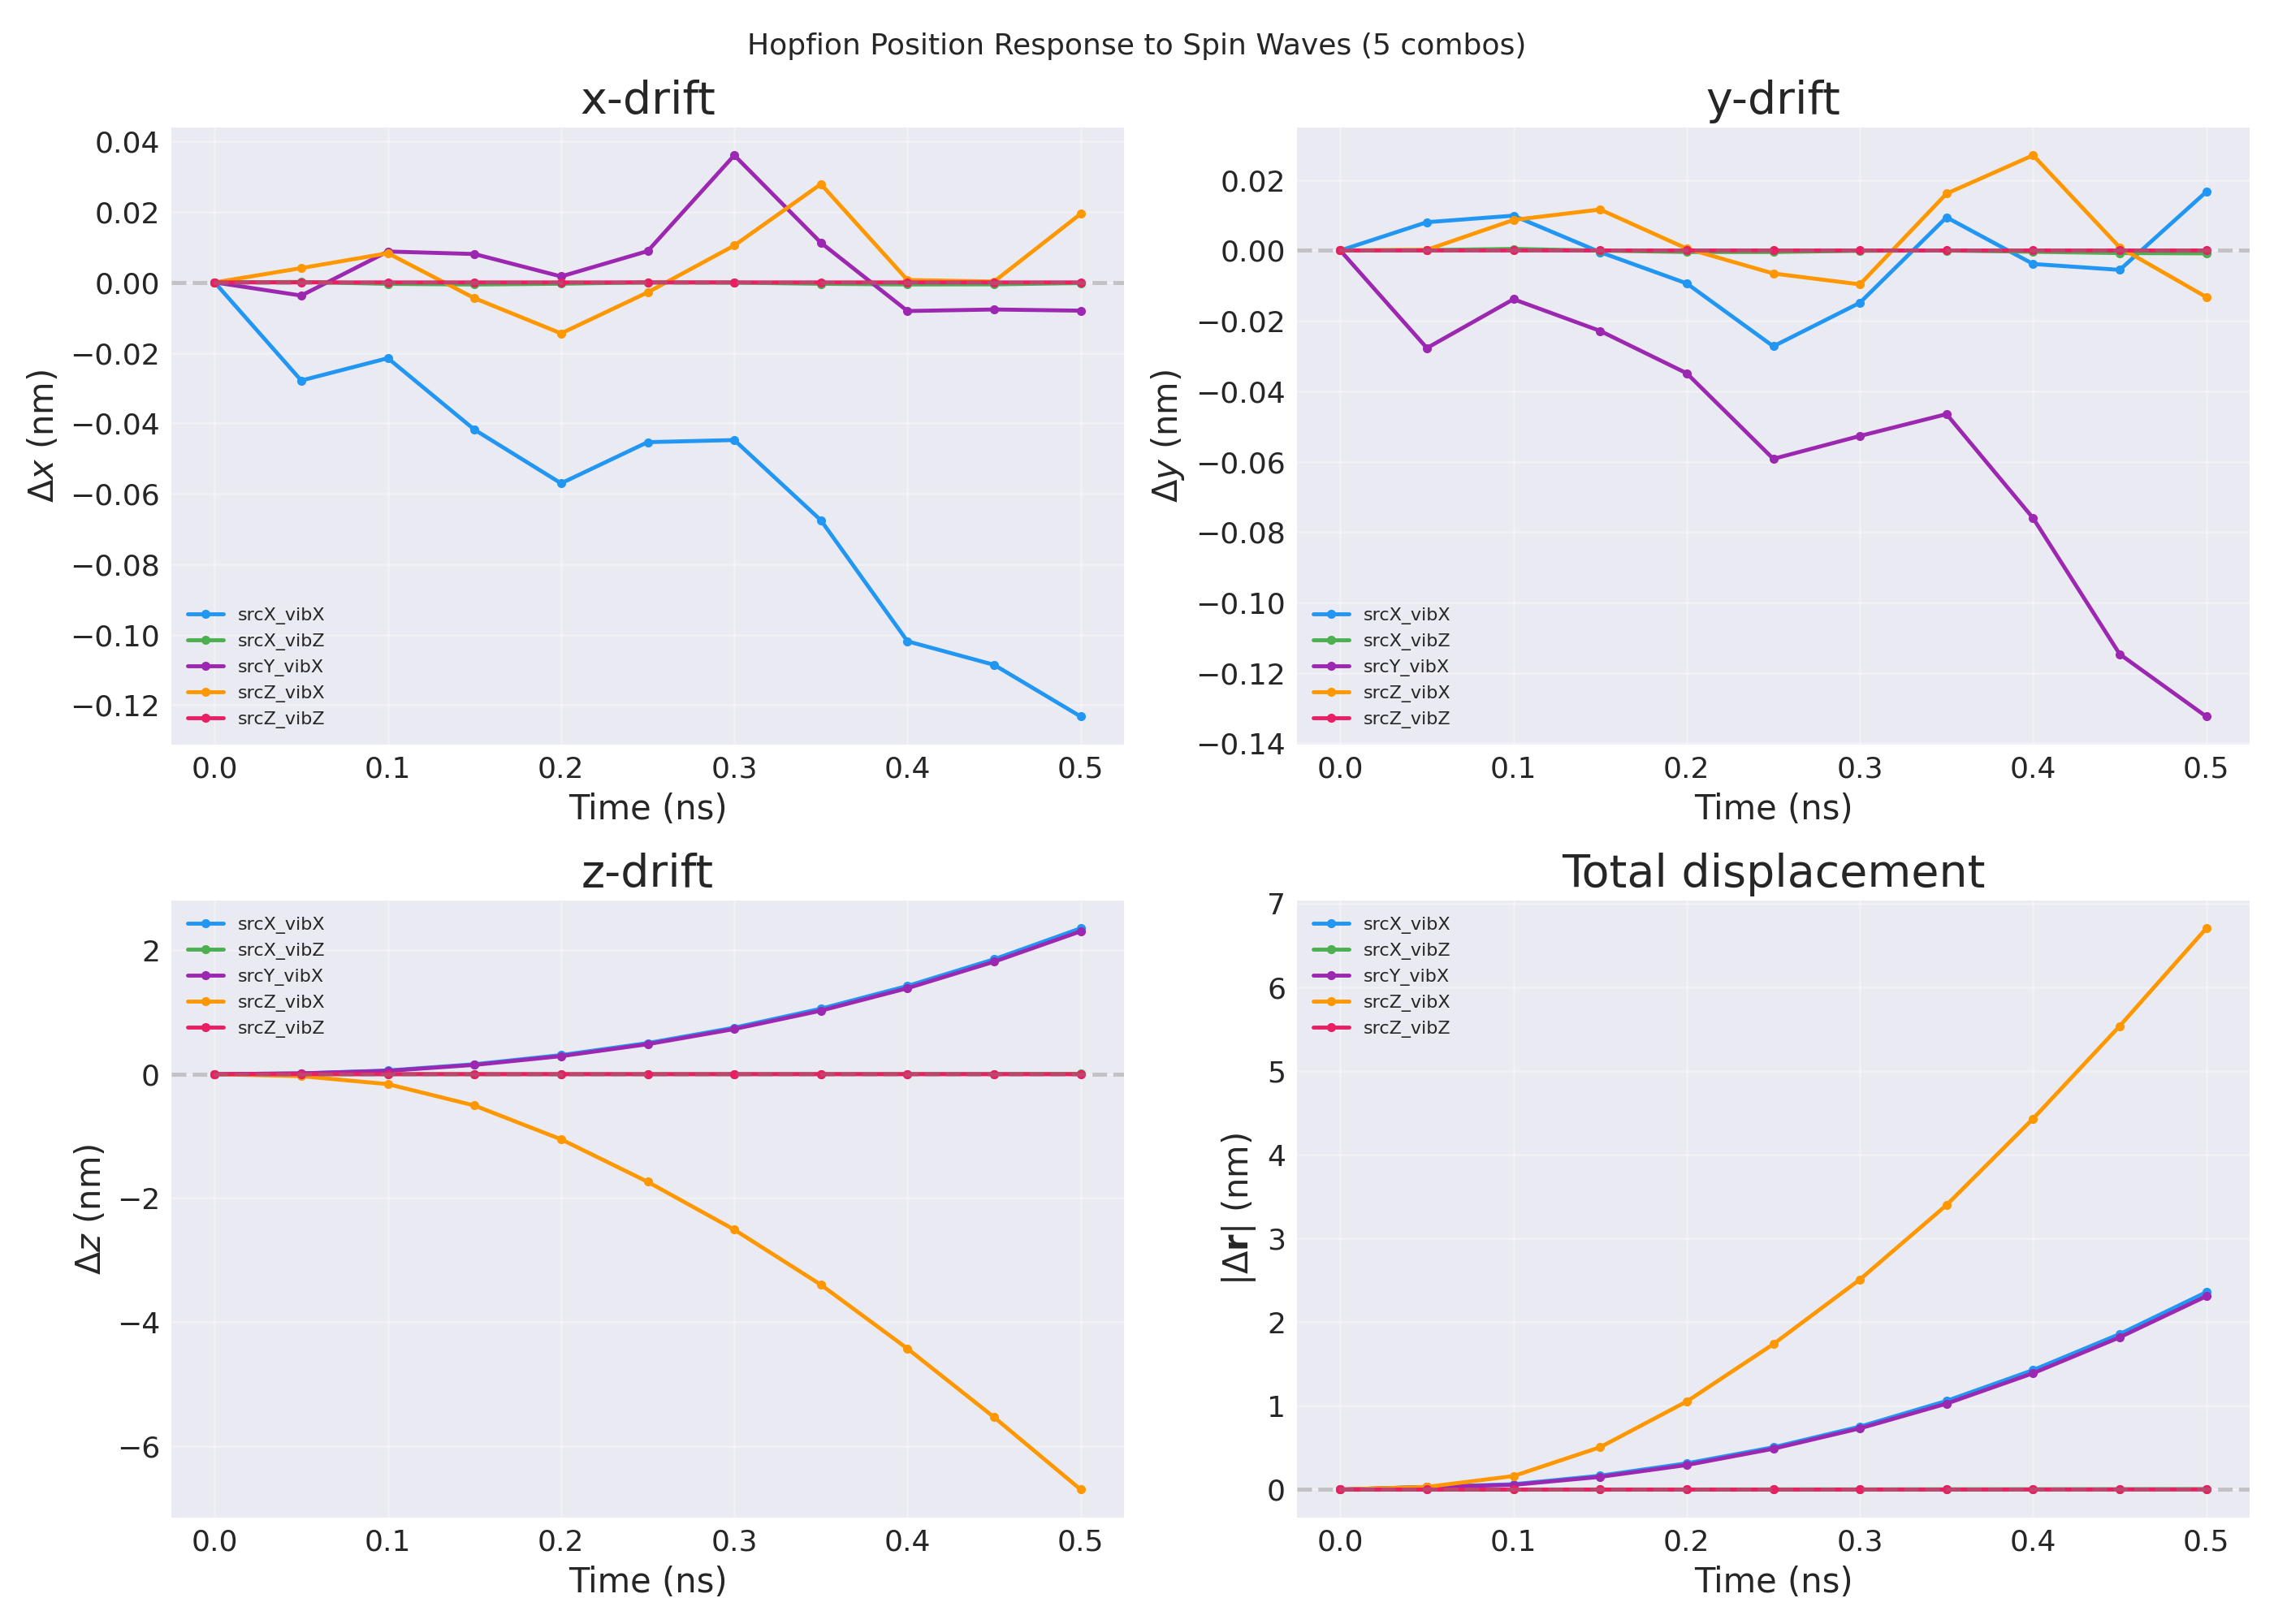
\includegraphics[width=0.95\textwidth]{figures/fig4-1_direction_selectivity.png}
  \caption{5 种驱动组合下 Hopfion 质心坐标随时间的演化。面内振荡（vibX）组合产生显著运动，面外振荡（vibZ）组合无响应}
  \label{fig:direction-selectivity}
\end{figure}

这些结果说明两点。\textbf{（1）振荡方向选择性}：只有面内振荡（$\hat{x}$ 方向）才能有效驱动 Hopfion 运动，面外振荡（$\hat{z}$ 方向）几乎没有效果。原因是 $\hat{z}$ 振荡保持了 Hopfion 的轴对称性，无法激发平动模式；而 $\hat{x}$ 振荡打破了面内对称性，提供了平动所需的线性动量。\textbf{（2）面内等价性}：srcX\_vibX 和 srcY\_vibX 的位移量几乎相同（$2.36$ vs $\SI{2.31}{nm}$），验证了 Hopfion 面内传播的各向同性，这与 Hopfion 的轴对称 $xy$ 平面旋转不变性一致。

另外，三个有效组合的运动方向有明显差异。srcX\_vibX 和 srcY\_vibX 驱动 Hopfion 沿 $+z$ 方向运动（垂直于传播方向），而 srcZ\_vibX 驱动 Hopfion 沿 $-z$ 方向运动（沿传播方向）。这一方向差异是后续实现双向轴向控制的物理基础。

\subsection{频率响应谱}
\label{subsec:freq-sweep}

确定了面内振荡（vibX）为有效驱动方式后，本文分别对面内传播（srcX）和轴向传播（srcZ）进行频率扫描，研究 Hopfion 运动的频率依赖性。

\subsubsection{面内传播 srcX 的频率响应}

以 srcX\_vibX 组合，固定 $B_0 = \SI{1}{T}$，在 $\SIrange{100}{1000}{GHz}$ 范围内以 $\SI{100}{GHz}$ 间距进行 10 个频率点的扫描。\cref{fig:srcX-motion-mode}展示了各频率下的 Hopfion 运动模式分类结果。

\begin{figure}[htbp]
  \centering
  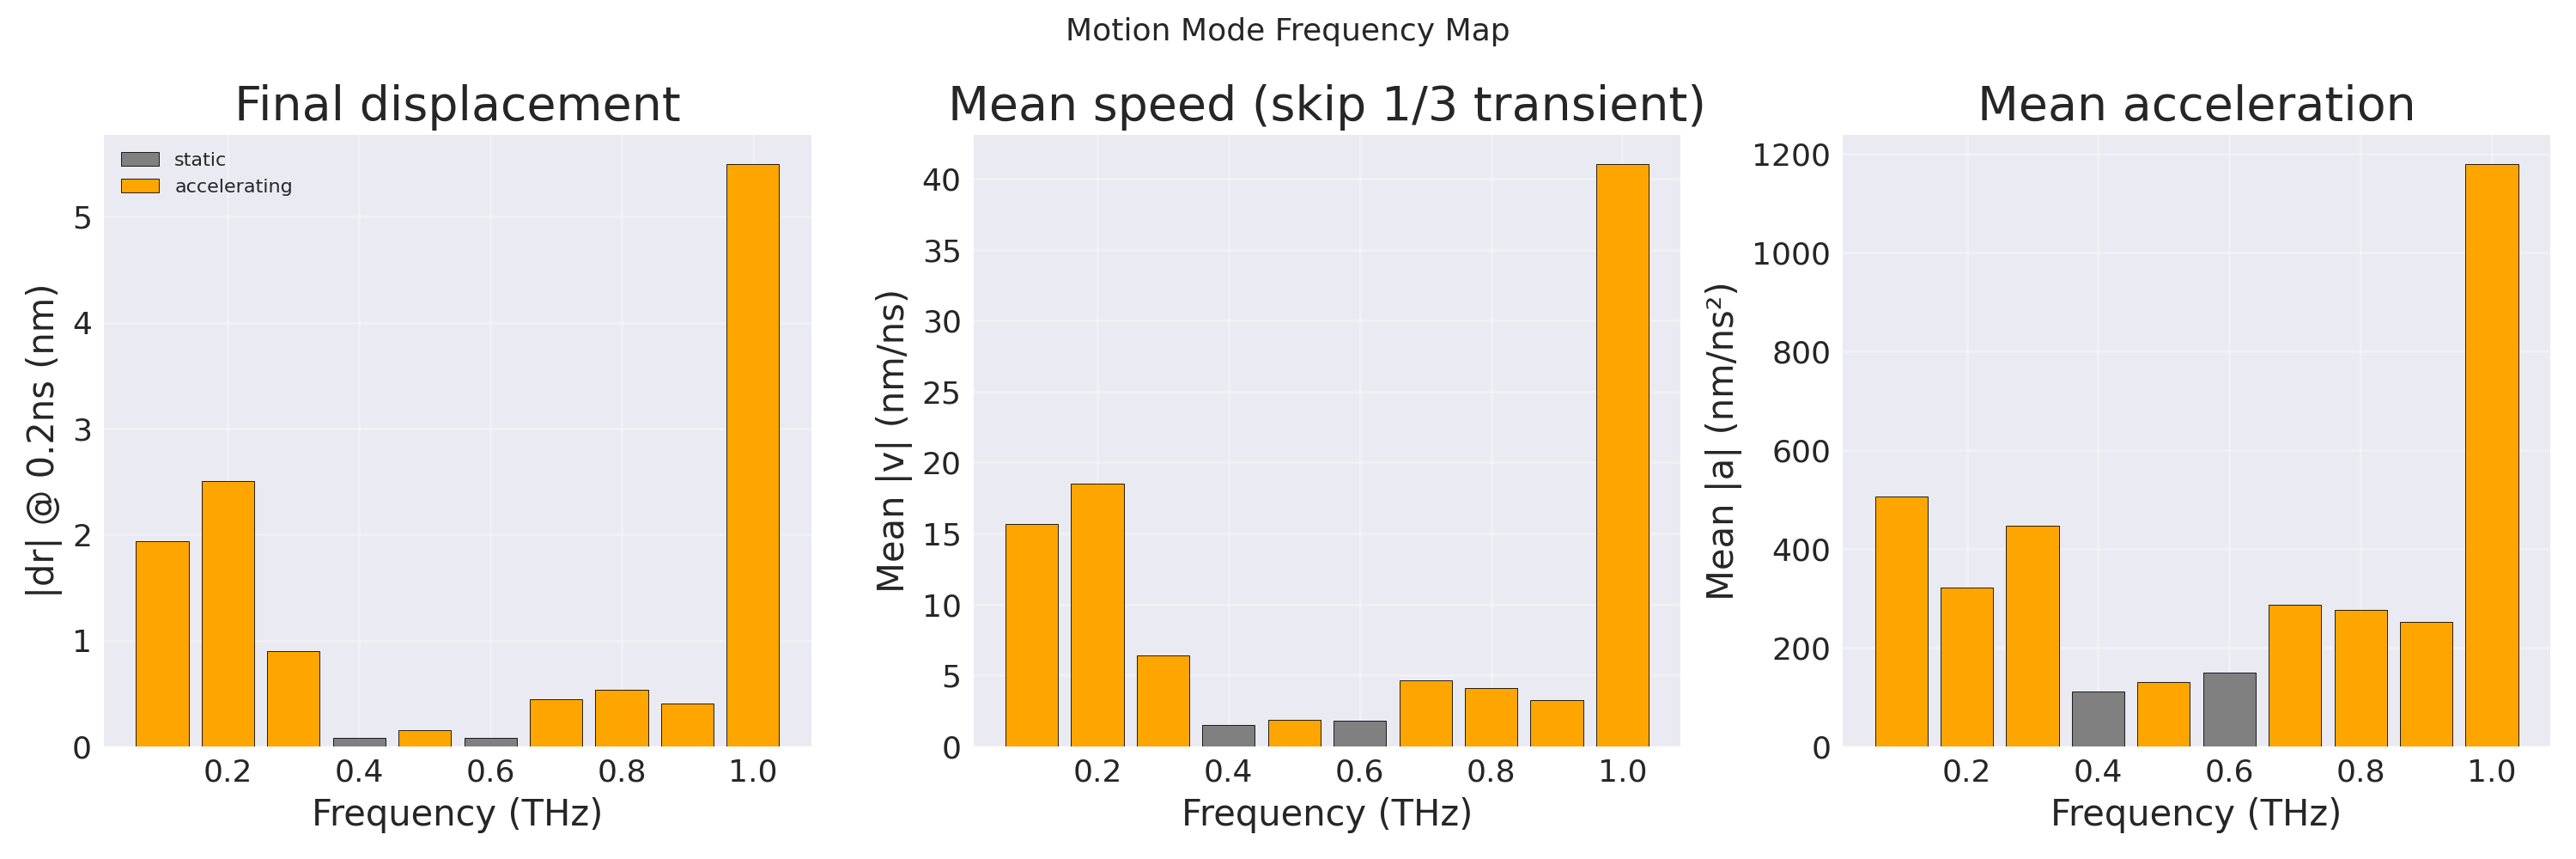
\includegraphics[width=0.95\textwidth]{figures/fig4-2_srcX_motion_mode.png}
  \caption{srcX 驱动 10 个频率点的运动模式分类。蓝色实线为 $z$ 方向位移 $\Delta z(t)$，红色虚线为运动模式拟合曲线}
  \label{fig:srcX-motion-mode}
\end{figure}

\begin{figure}[htbp]
  \centering
  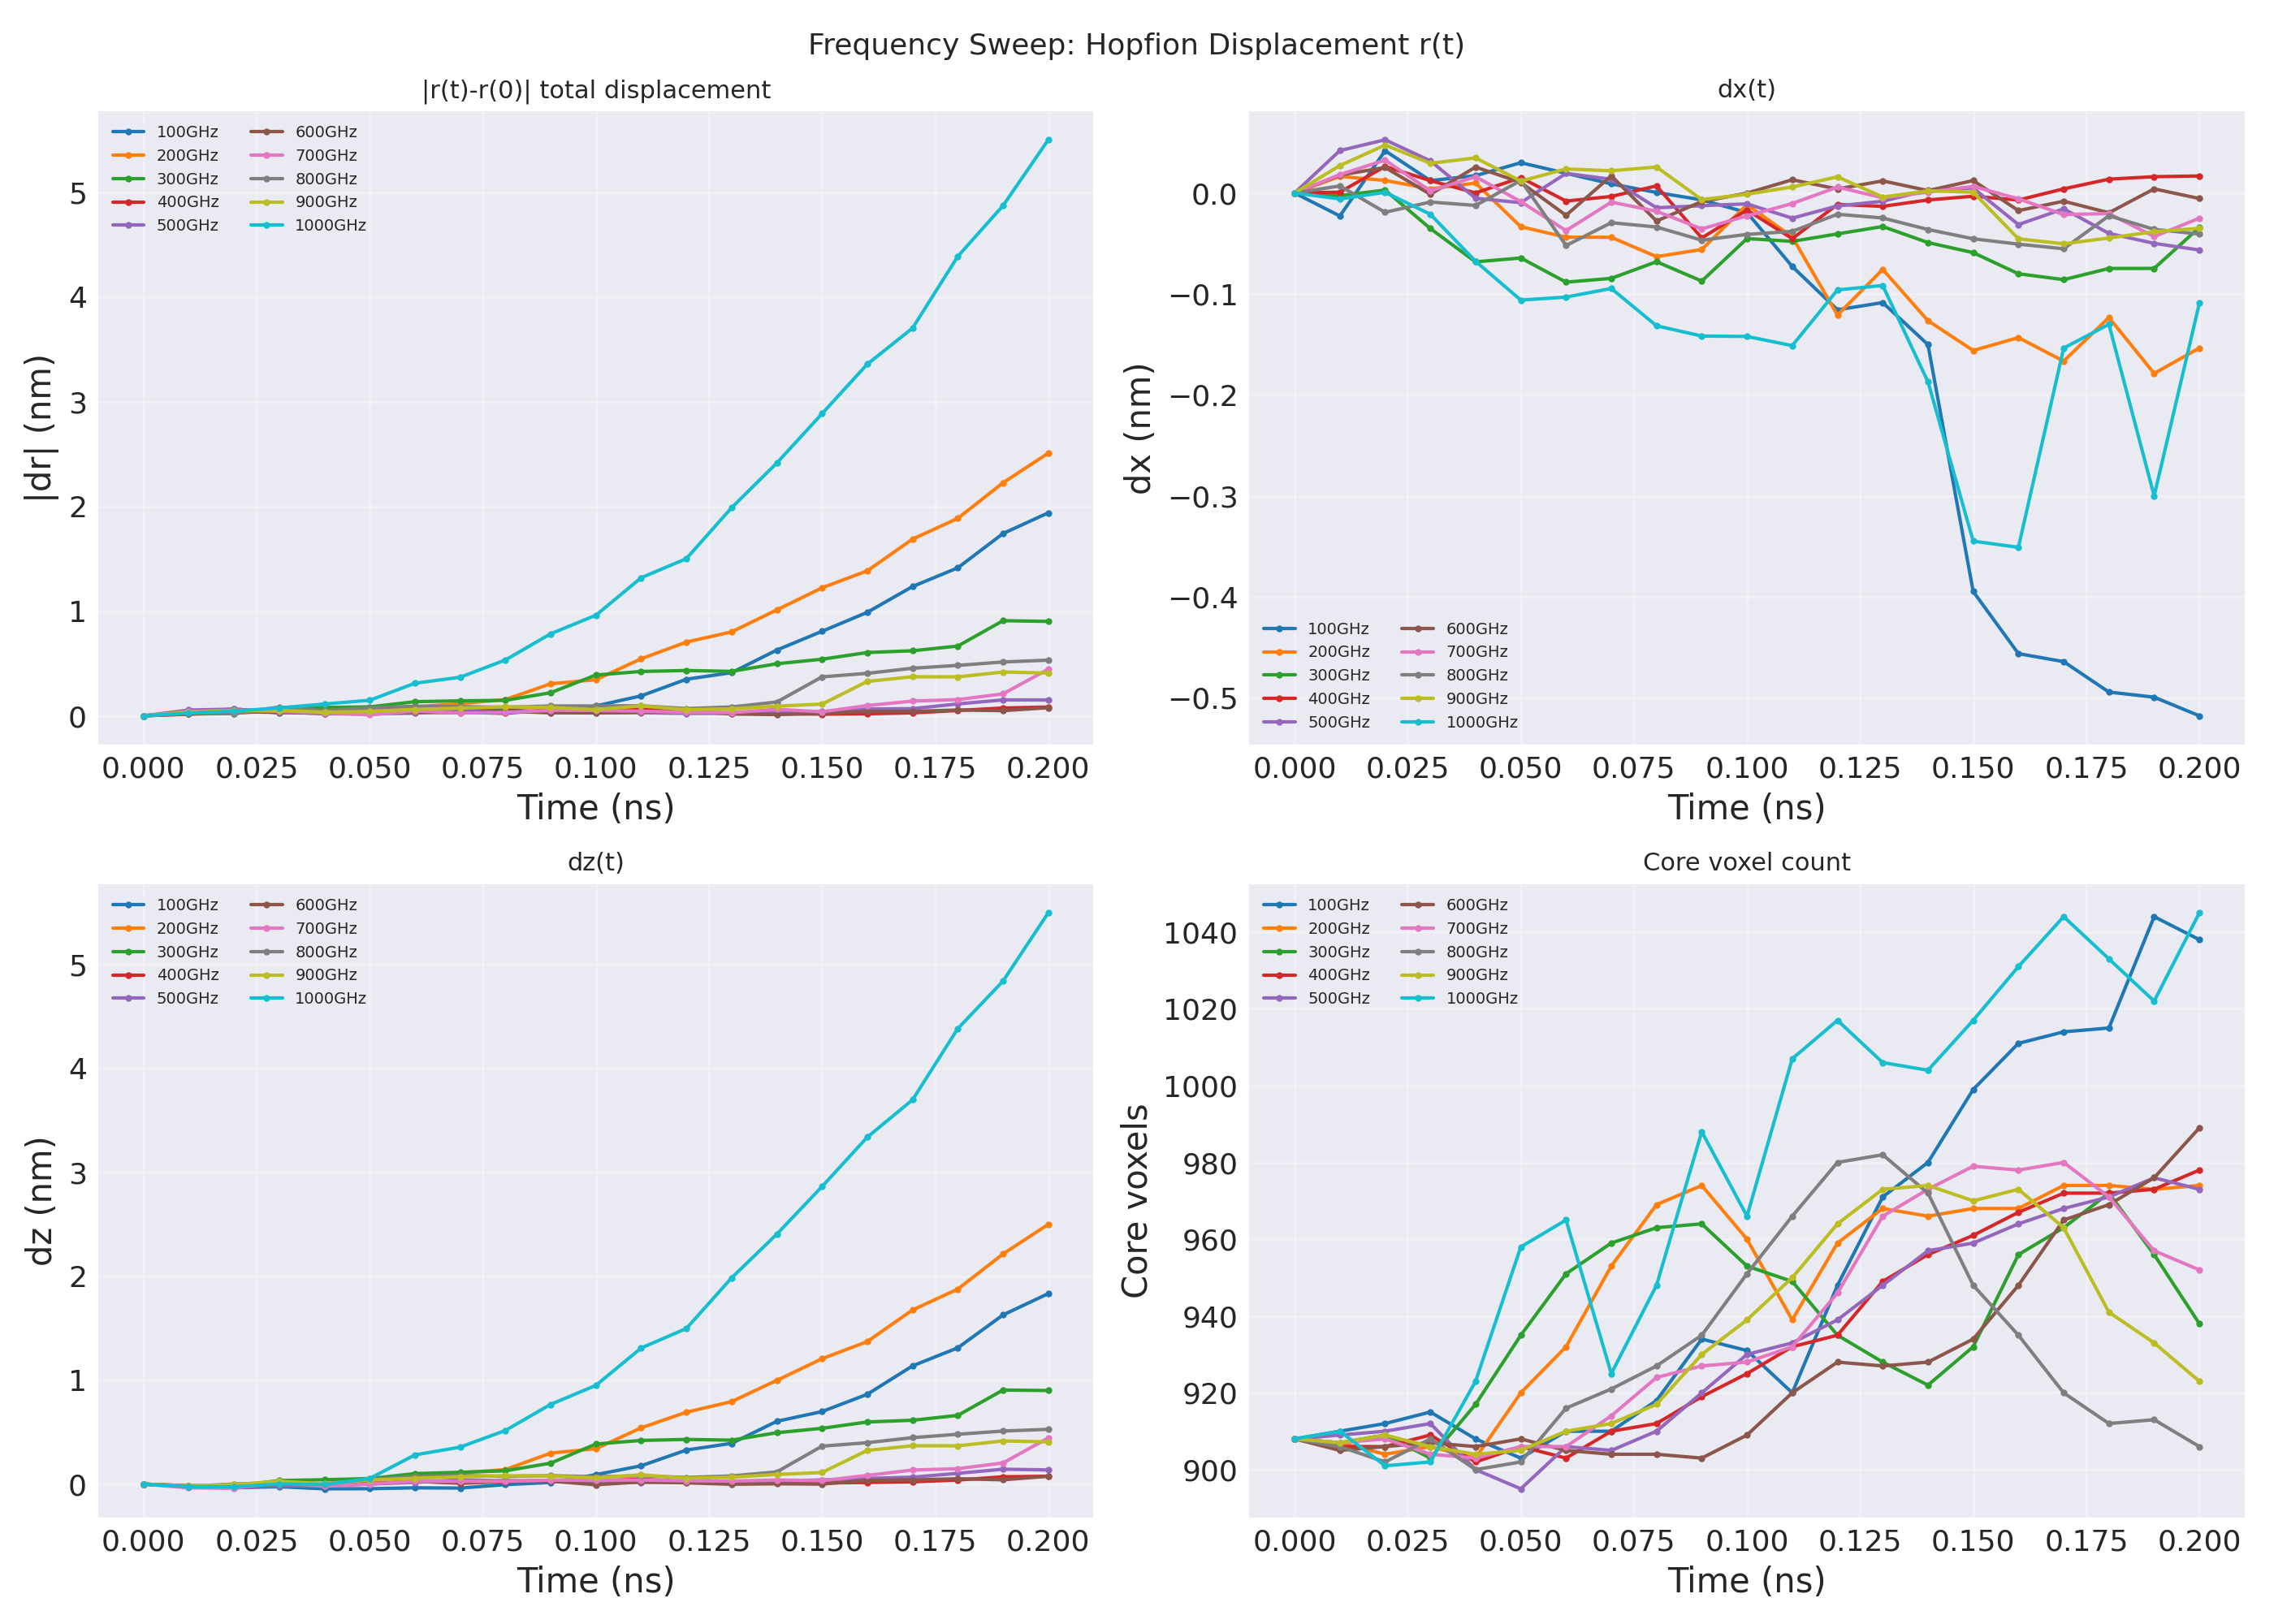
\includegraphics[width=0.95\textwidth]{figures/fig4-3_srcX_displacement.png}
  \caption{srcX 驱动下 Hopfion 位移 $|\Delta r|$ 和平均速度 $\bar{v}$ 随频率的变化。$\SI{1000}{GHz}$ 为最强响应点，$\SIrange{400}{600}{GHz}$ 为死区}
  \label{fig:srcX-displacement}
\end{figure}

结果呈现出强烈的频率选择性。\textbf{有效驱动区}包括低频段 $\SIrange{100}{200}{GHz}$（$|\Delta r| = \SIrange{1.94}{2.51}{nm}$）和高频段 $\SI{1000}{GHz}$（$|\Delta r| = \SI{5.50}{nm}$，为全频段最强）。\textbf{死区}为 $\SIrange{400}{600}{GHz}$（$|\Delta r| < \SI{0.15}{nm}$），Hopfion 几乎不动。中间频段 $\SIrange{700}{900}{GHz}$ 响应中等（$\SIrange{0.4}{0.5}{nm}$）。在所有频率下 Hopfion 均沿 $+z$ 方向运动，运动方向不随频率改变。

\subsubsection{轴向传播 srcZ 的频率响应}

srcZ 驱动的频率扫描覆盖 $\SIrange{25}{1500}{GHz}$ 共 20 个频率点（粗扫 + 细化）。结果如\cref{fig:srcZ-freq-response}和\cref{fig:srcZ-direction-map}所示。

\begin{figure}[htbp]
  \centering
  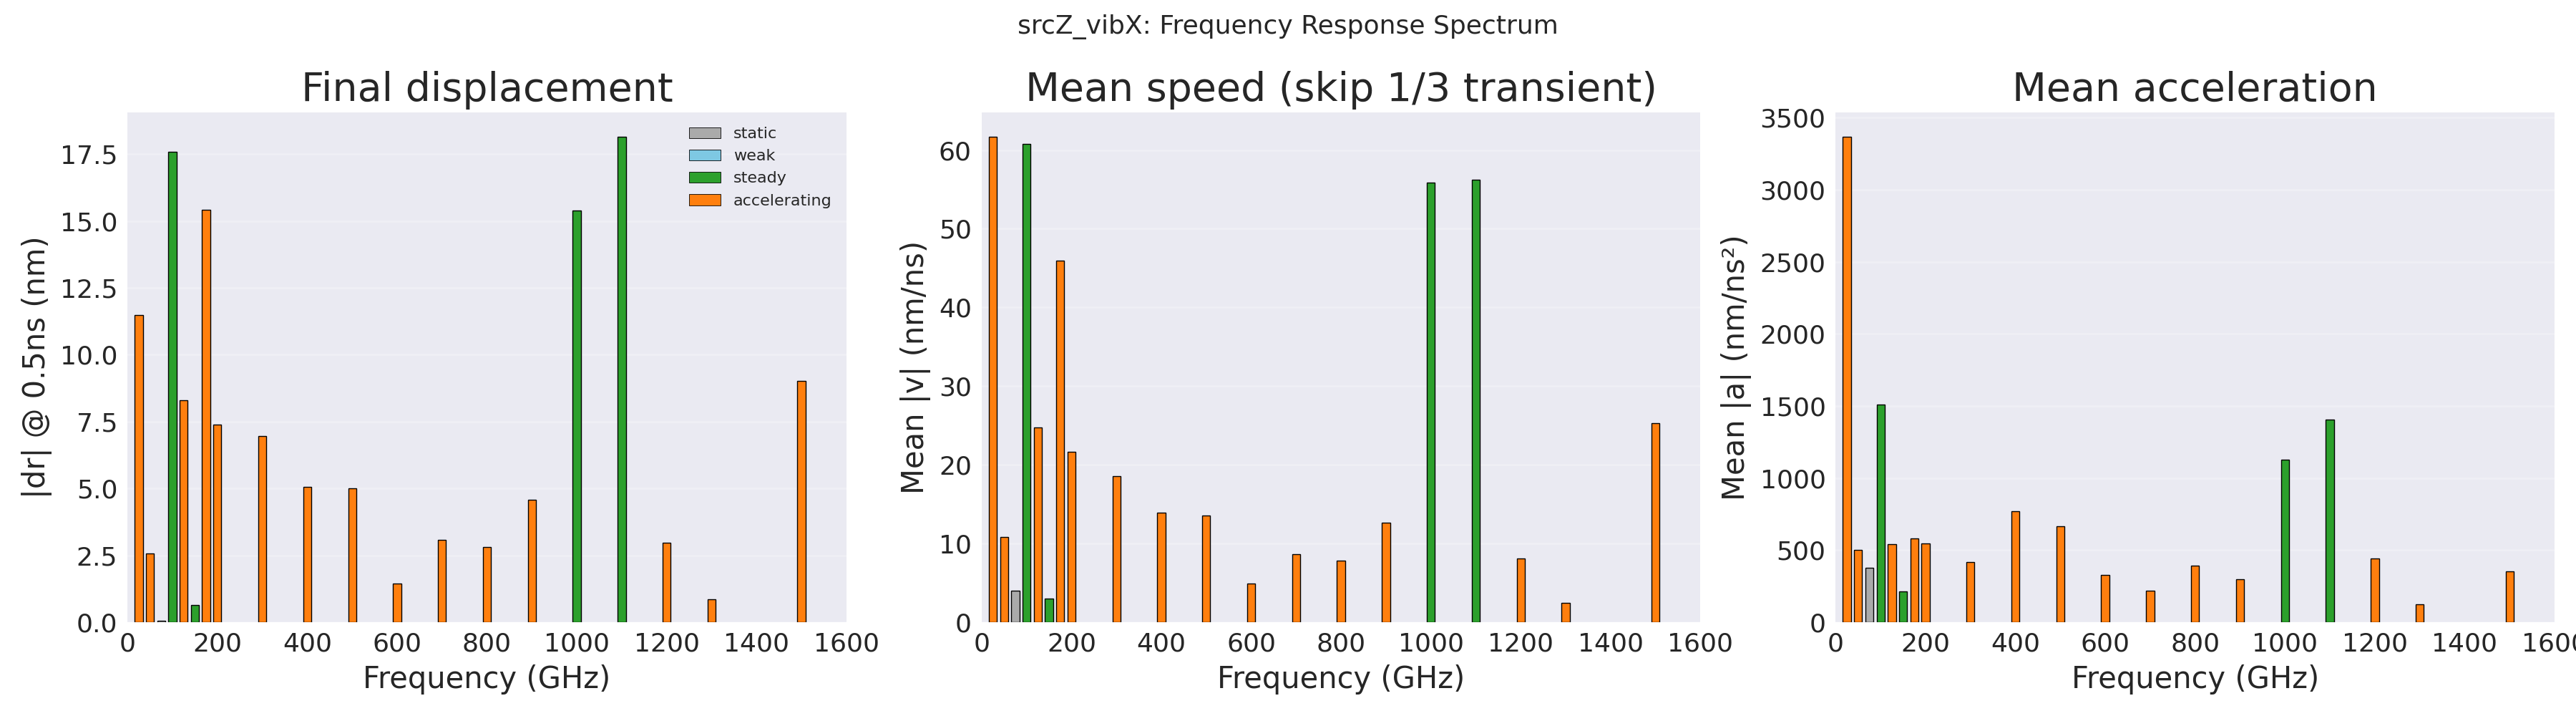
\includegraphics[width=0.95\textwidth]{figures/fig4-4_srcZ_freq_response.png}
  \caption{srcZ 驱动下 20 个频率点的 Hopfion 位移谱。$\SI{1100}{GHz}$ 为全频段最强响应（$|\Delta r| = \SI{18.1}{nm}$），$\SI{100}{GHz}$ 为唯一 $+z$ 异常点}
  \label{fig:srcZ-freq-response}
\end{figure}

\begin{figure}[htbp]
  \centering
  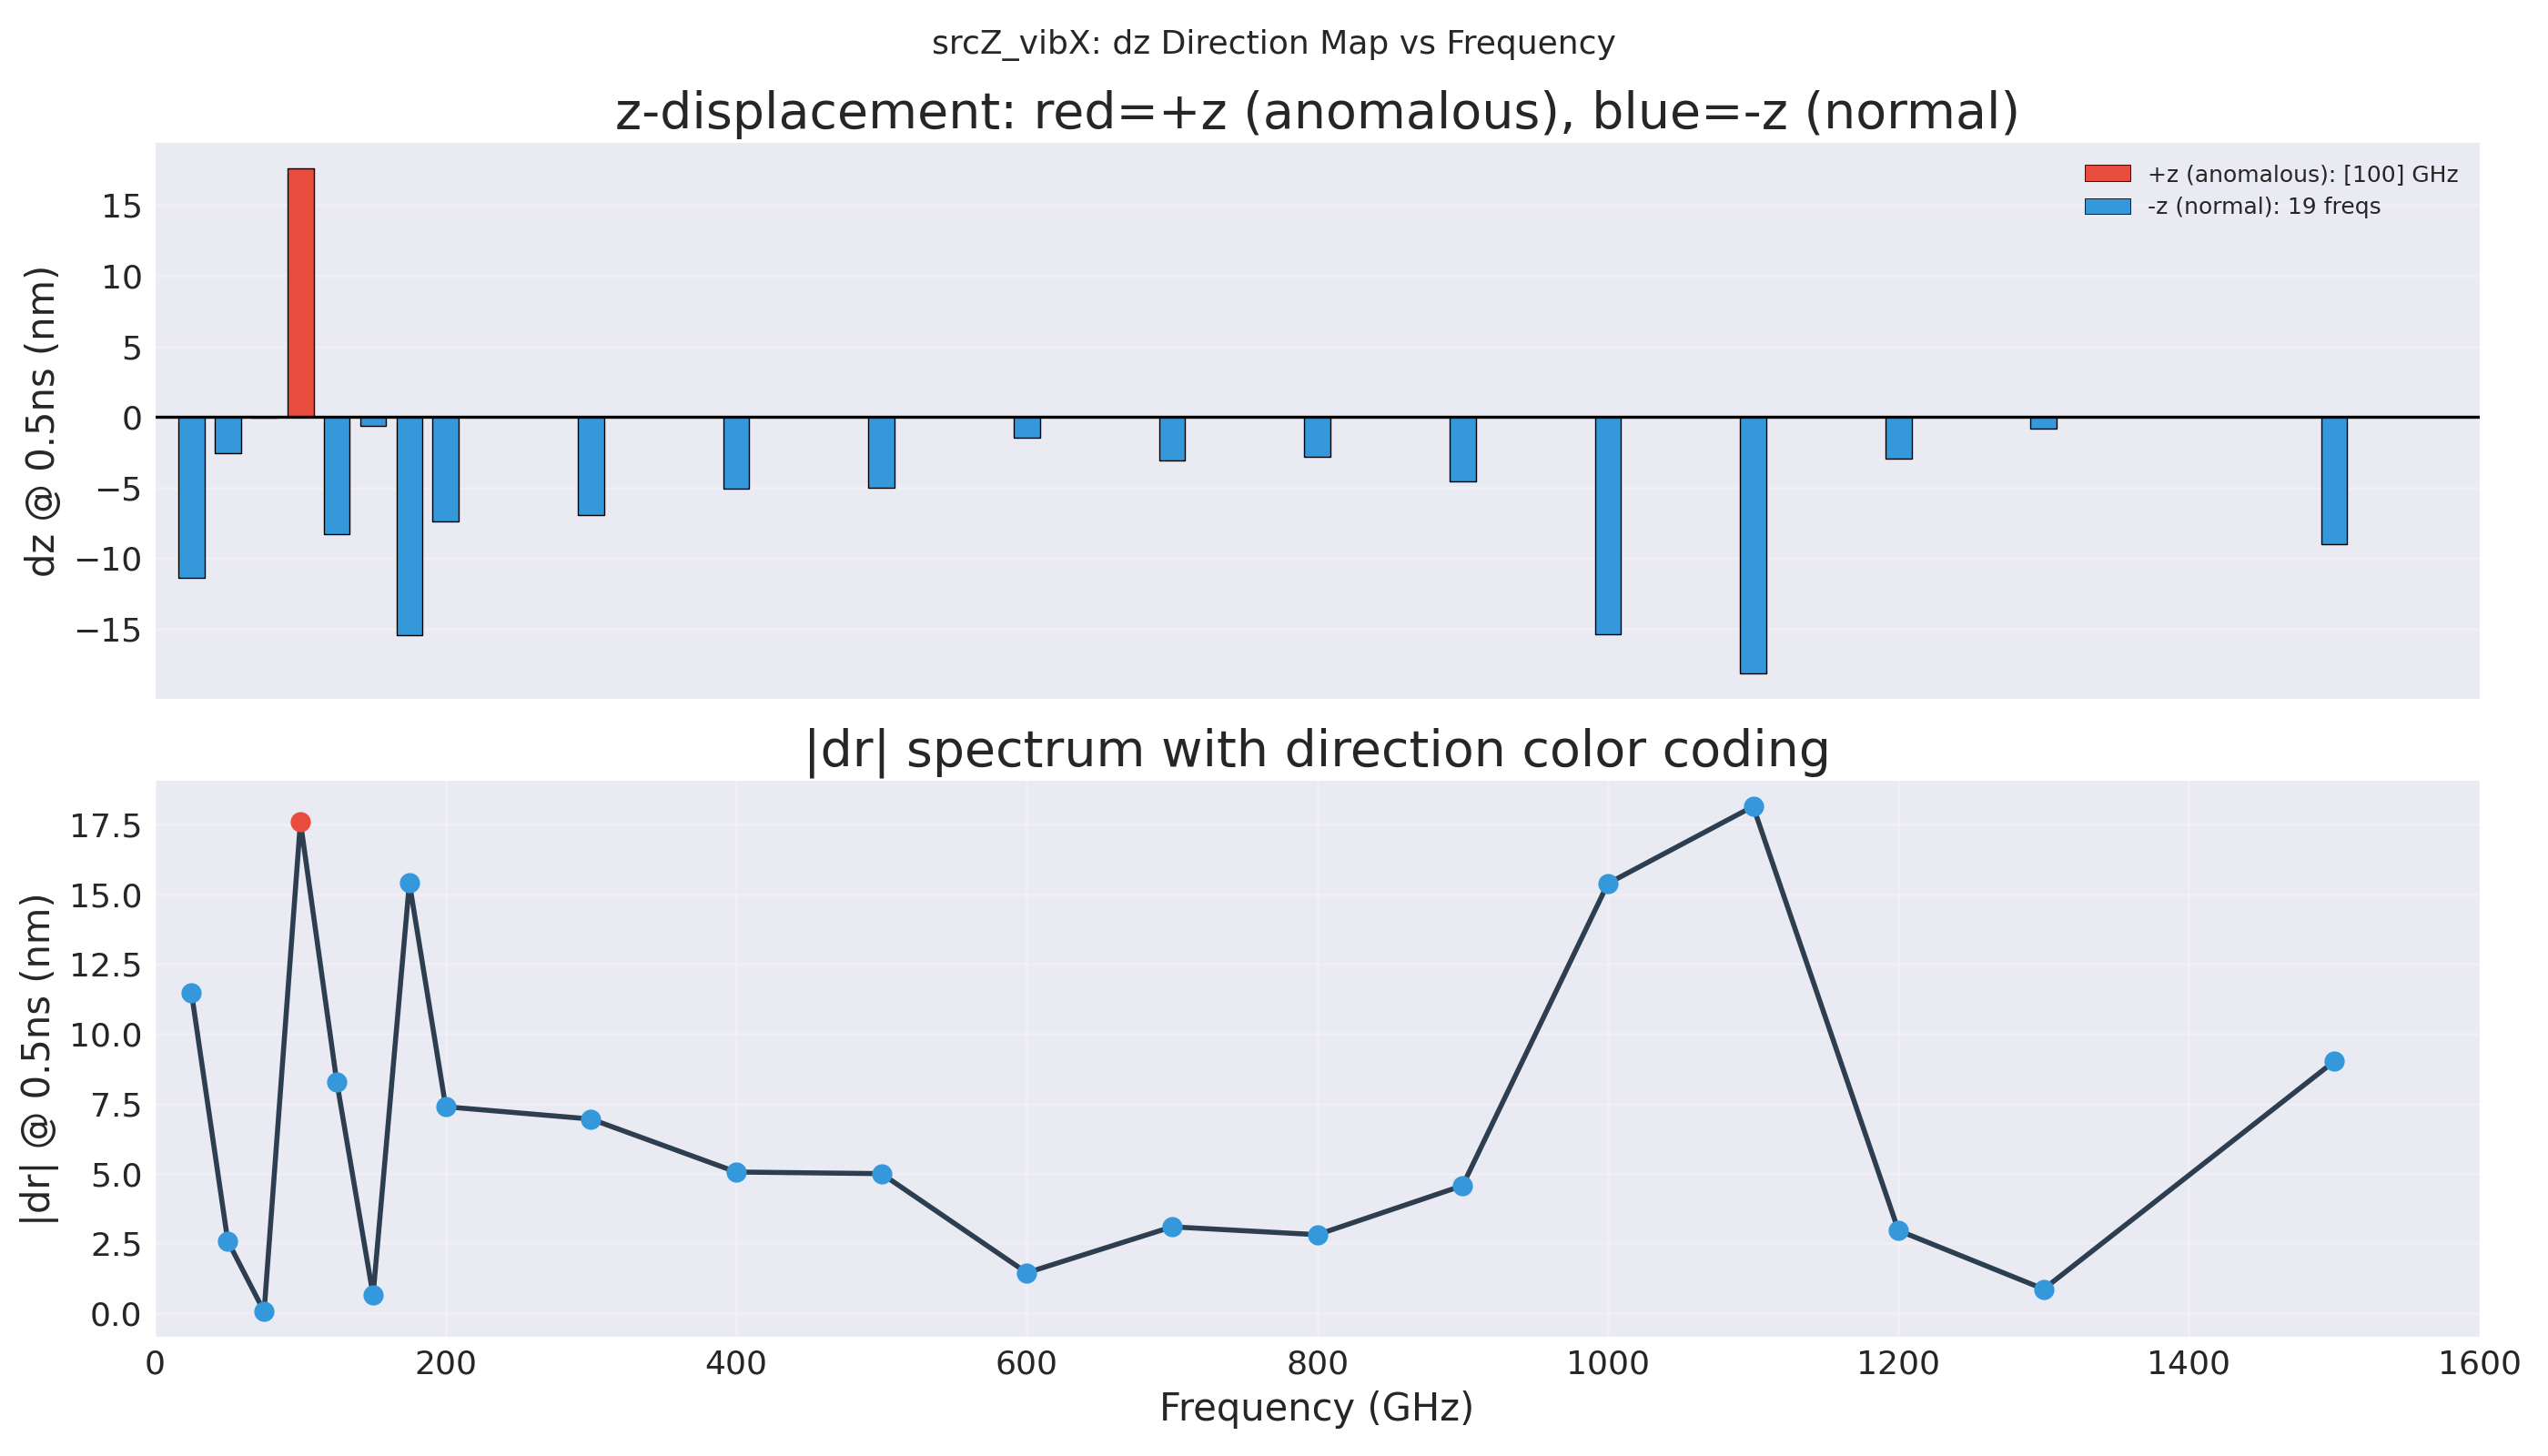
\includegraphics[width=0.95\textwidth]{figures/fig4-5_srcZ_direction_map.png}
  \caption{srcZ 驱动方向图。除 $\SI{100}{GHz}$ 外，所有频率均驱动 Hopfion 沿 $-z$ 方向运动}
  \label{fig:srcZ-direction-map}
\end{figure}

srcZ 展现出与 srcX 截然不同的频率响应特征：（1）\textbf{方向异常}：$\SI{100}{GHz}$ 是唯一驱动 Hopfion 沿 $+z$（朝向源）运动的频率（$\Delta z = +\SI{17.6}{nm}$），其余 19 个频率均驱动 $-z$（远离源）运动。（2）\textbf{共振谱多峰}：$\SI{1100}{GHz}$ 为全局最强共振（$|\Delta r| = \SI{18.1}{nm}$, $\bar{v} = \SI{56.3}{nm/ns}$），$\SI{100}{GHz}$（$\SI{17.6}{nm}$）和 $\SI{1000}{GHz}$（$\SI{15.4}{nm}$）为次强峰。死区位于 $\SI{75}{GHz}$、$\SI{150}{GHz}$、$\SI{600}{GHz}$ 和 $\SI{1300}{GHz}$。（3）\textbf{运动模式}：强响应点呈现"steady"模式（匀速运动），弱响应点为"accelerating"模式。

srcX 和 srcZ 的频率响应差异反映了不同自旋波传播方向与 Hopfion 内部模式的耦合机制不同。面内传播的自旋波主要激发面内平动模式（$+z$ Hall 运动），而轴向传播的自旋波直接耦合轴向平动模式（$-z$ 运动），两者的共振频率分布也不一致。

\subsection{能量吸收谱}
\label{subsec:energy-absorption}

为定量表征 Hopfion 与自旋波的耦合强度，从仿真记录的总能量 $E_{\text{total}}(t)$ 中提取能量吸收率 $\mathrm{d}E/\mathrm{d}t$。对每个频率点取 $0.3T$–$T$ 时间段（避开初始瞬态）进行线性拟合，斜率即为平均能量吸收率。

\begin{figure}[htbp]
  \centering
  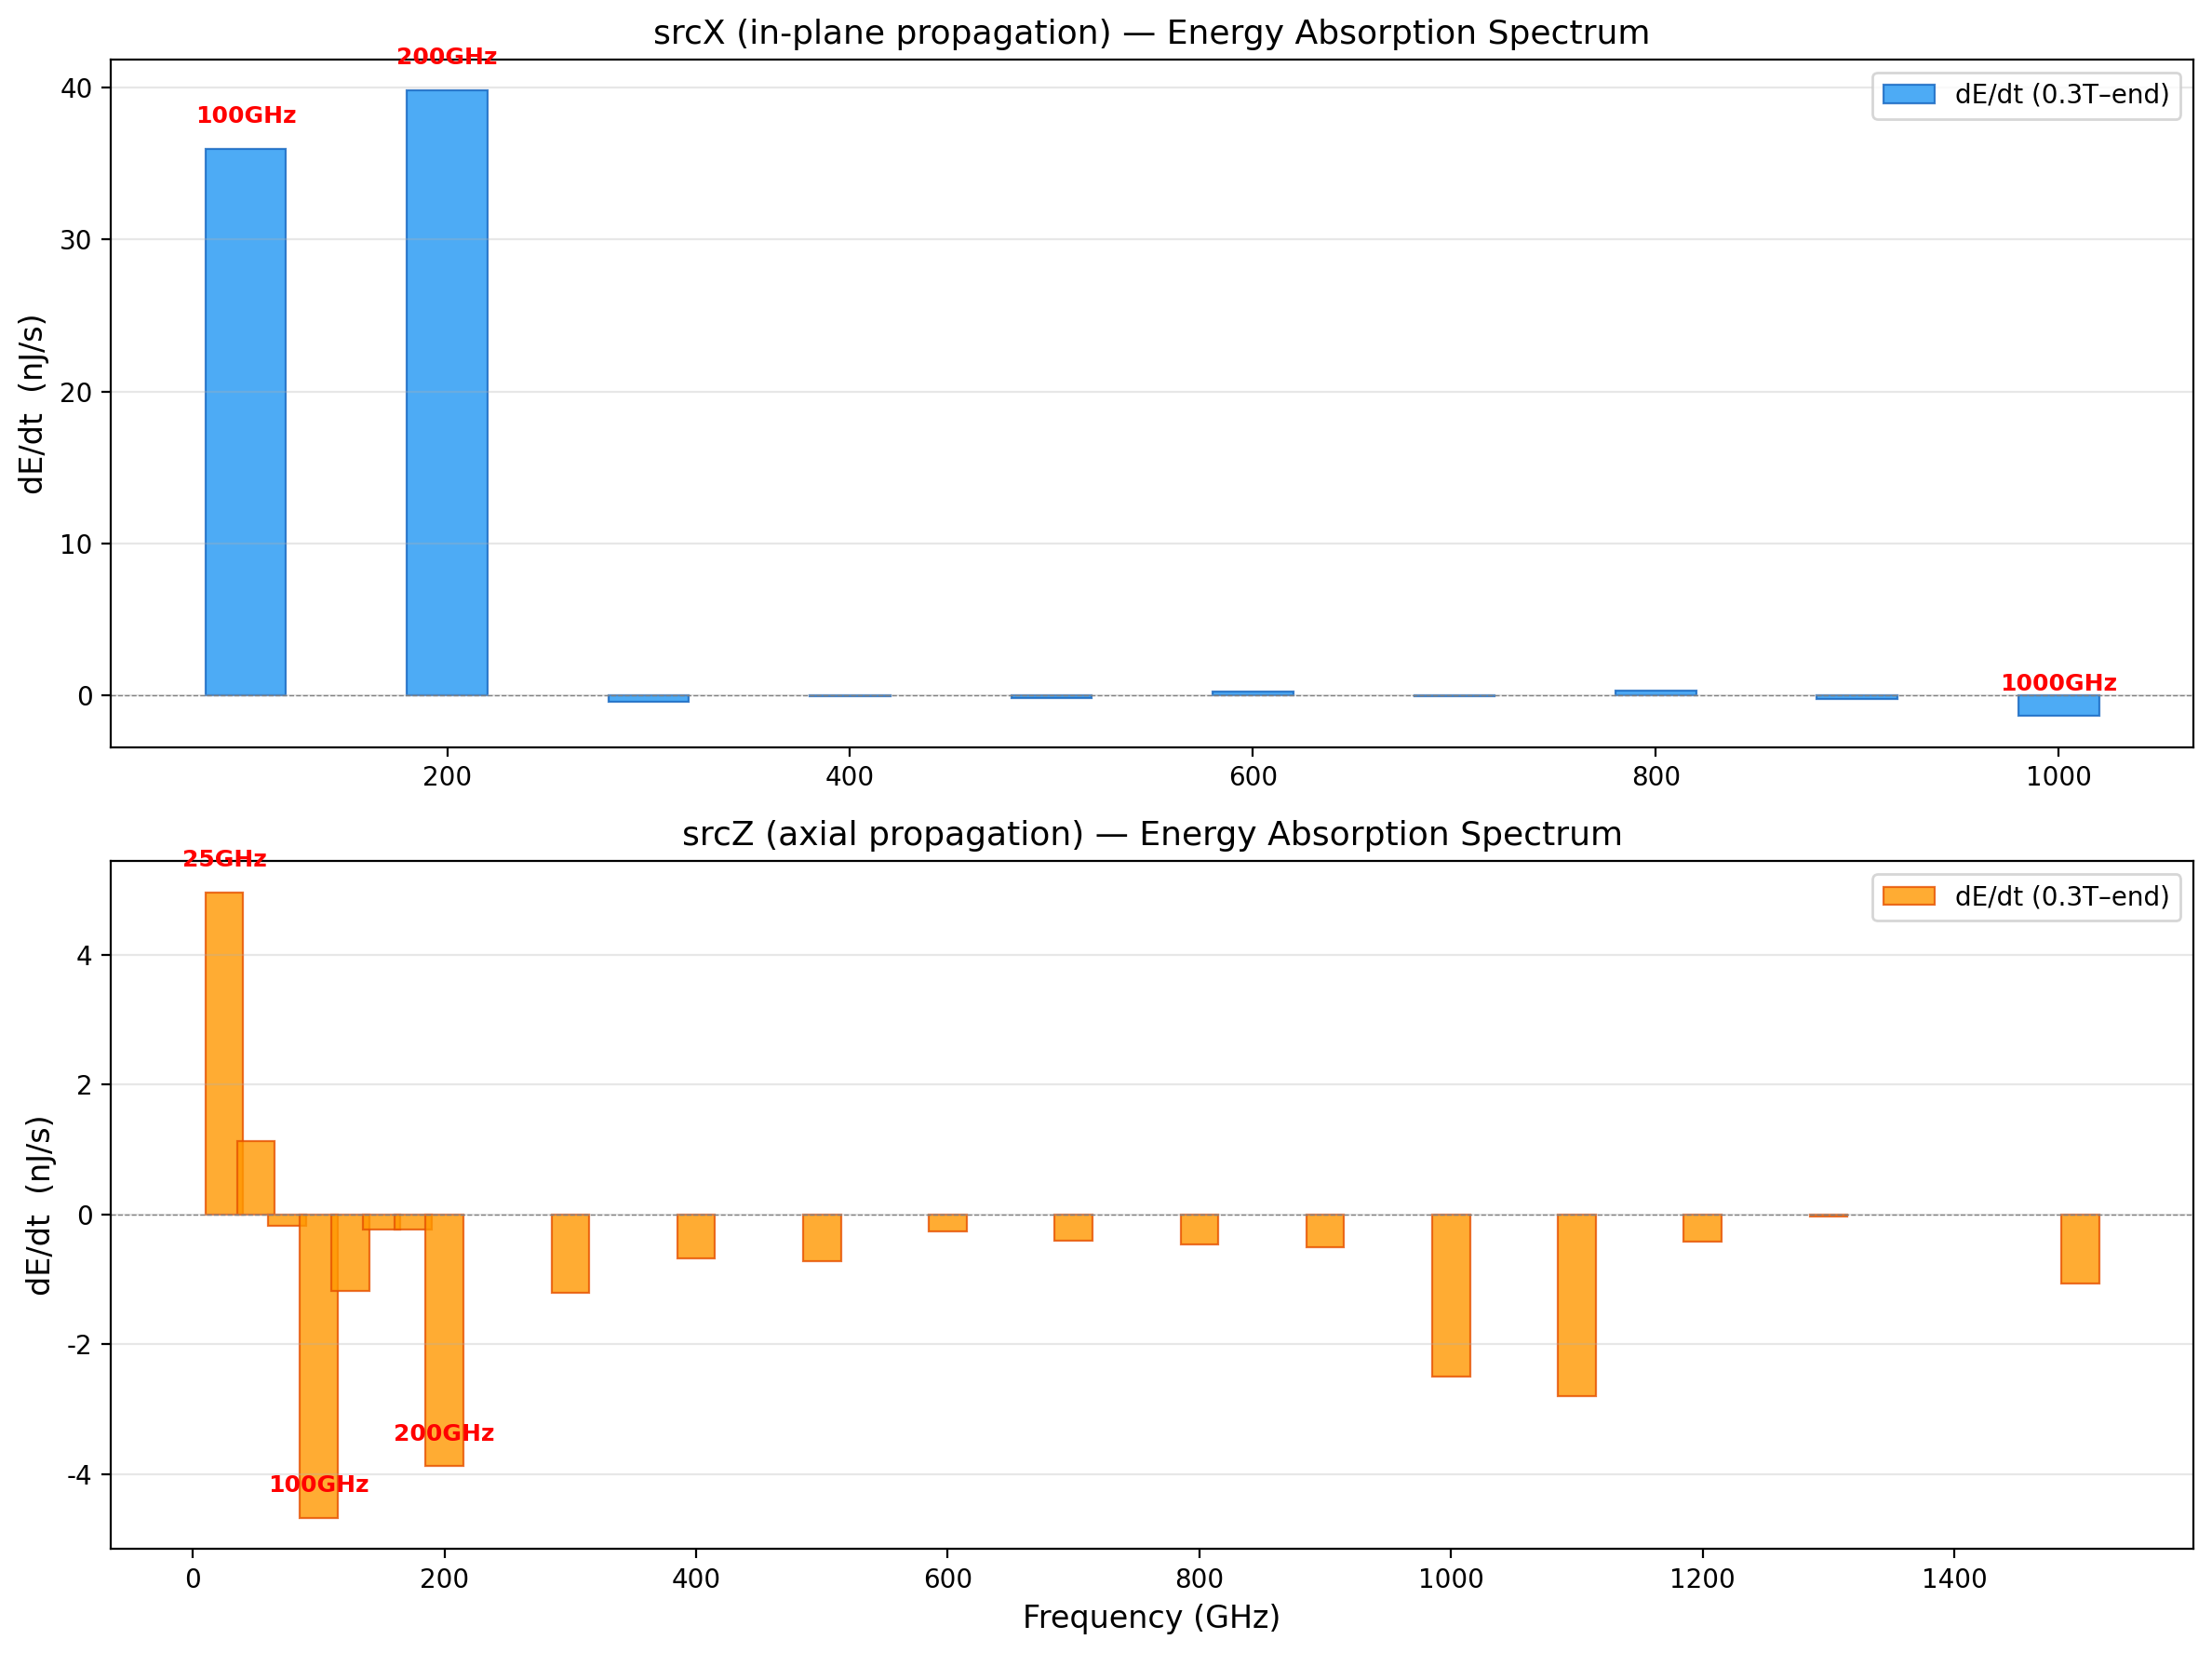
\includegraphics[width=0.95\textwidth]{figures/fig4-6_energy_absorption.png}
  \caption{能量吸收谱 $\mathrm{d}E/\mathrm{d}t$ vs $f$。上：srcX（面内传播），$\SI{200}{GHz}$ 为能量吸收最强点；下：srcZ（轴向传播），$\SI{100}{GHz}$ 吸收最强}
  \label{fig:energy-absorption}
\end{figure}

如\cref{fig:energy-absorption}所示，srcX 的能量吸收谱以 $\SI{100}{GHz}$（$\SI{36.0}{nJ/s}$）和 $\SI{200}{GHz}$（$\SI{39.8}{nJ/s}$, $R^2 = 0.986$）为双峰，$\SIrange{300}{800}{GHz}$ 吸收率接近零（$< \SI{0.5}{nJ/s}$），与位移谱中 $\SIrange{400}{600}{GHz}$ 死区一致。srcZ 的能量吸收谱呈非对称多峰结构，$\SI{100}{GHz}$（$-\SI{4.67}{nJ/s}$，负号表示系统释放能量至外部驱动场）的绝对值最大，$\SIrange{400}{900}{GHz}$ 维持稳定吸收（$\SIrange{0.3}{0.7}{nJ/s}$）。

能量吸收谱与位移谱的对比揭示：（1）高能量吸收不一定对应大位移。例如 srcX@$\SI{200}{GHz}$ 的能量吸收率最高，但位移（$\SI{2.51}{nm}$）远不及 $\SI{1000}{GHz}$（$\SI{5.50}{nm}$），说明 $\SI{1000}{GHz}$ 模式的能量-运动转换效率更高。（2）srcZ@$\SI{100}{GHz}$ 的负能量吸收率与其 $+z$ 异常运动方向关联，暗示该模式可能涉及不同于其他频率的耦合机制。

\subsection{幅度标度律}
\label{subsec:amplitude-scaling}

本文固定 srcX\_vibX 组合和 $f = \SI{440}{GHz}$，在 $B_0 = \SIrange{0.05}{2.0}{T}$ 范围内进行 6 个幅度点的扫描，研究 Hopfion 运动速度与驱动幅度的定量关系。

\begin{figure}[htbp]
  \centering
  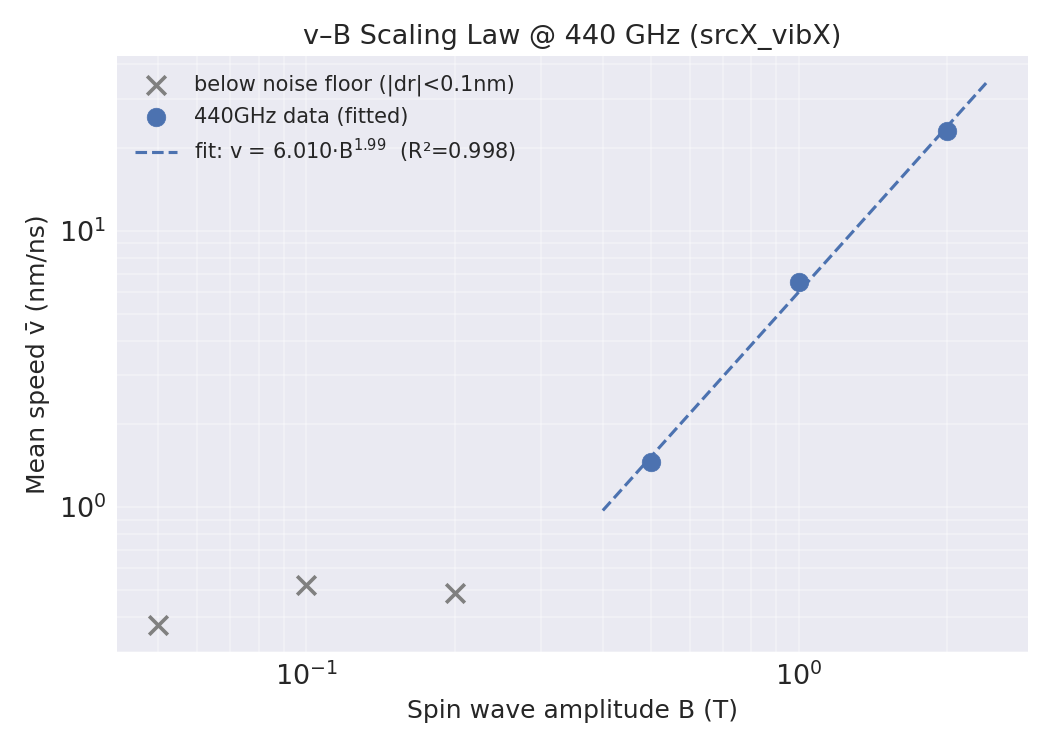
\includegraphics[width=0.95\textwidth]{figures/fig4-7_amplitude_scaling.png}
  \caption{Hopfion 平均速度 $\bar{v}$ 与自旋波幅度 $B_0$ 的关系（log-log 坐标）。$B_0 \geq \SI{0.5}{T}$ 时拟合得 $\bar{v} \propto B_0^{1.99}$，$R^2 = 0.998$}
  \label{fig:amplitude-scaling}
\end{figure}

\begin{figure}[htbp]
  \centering
  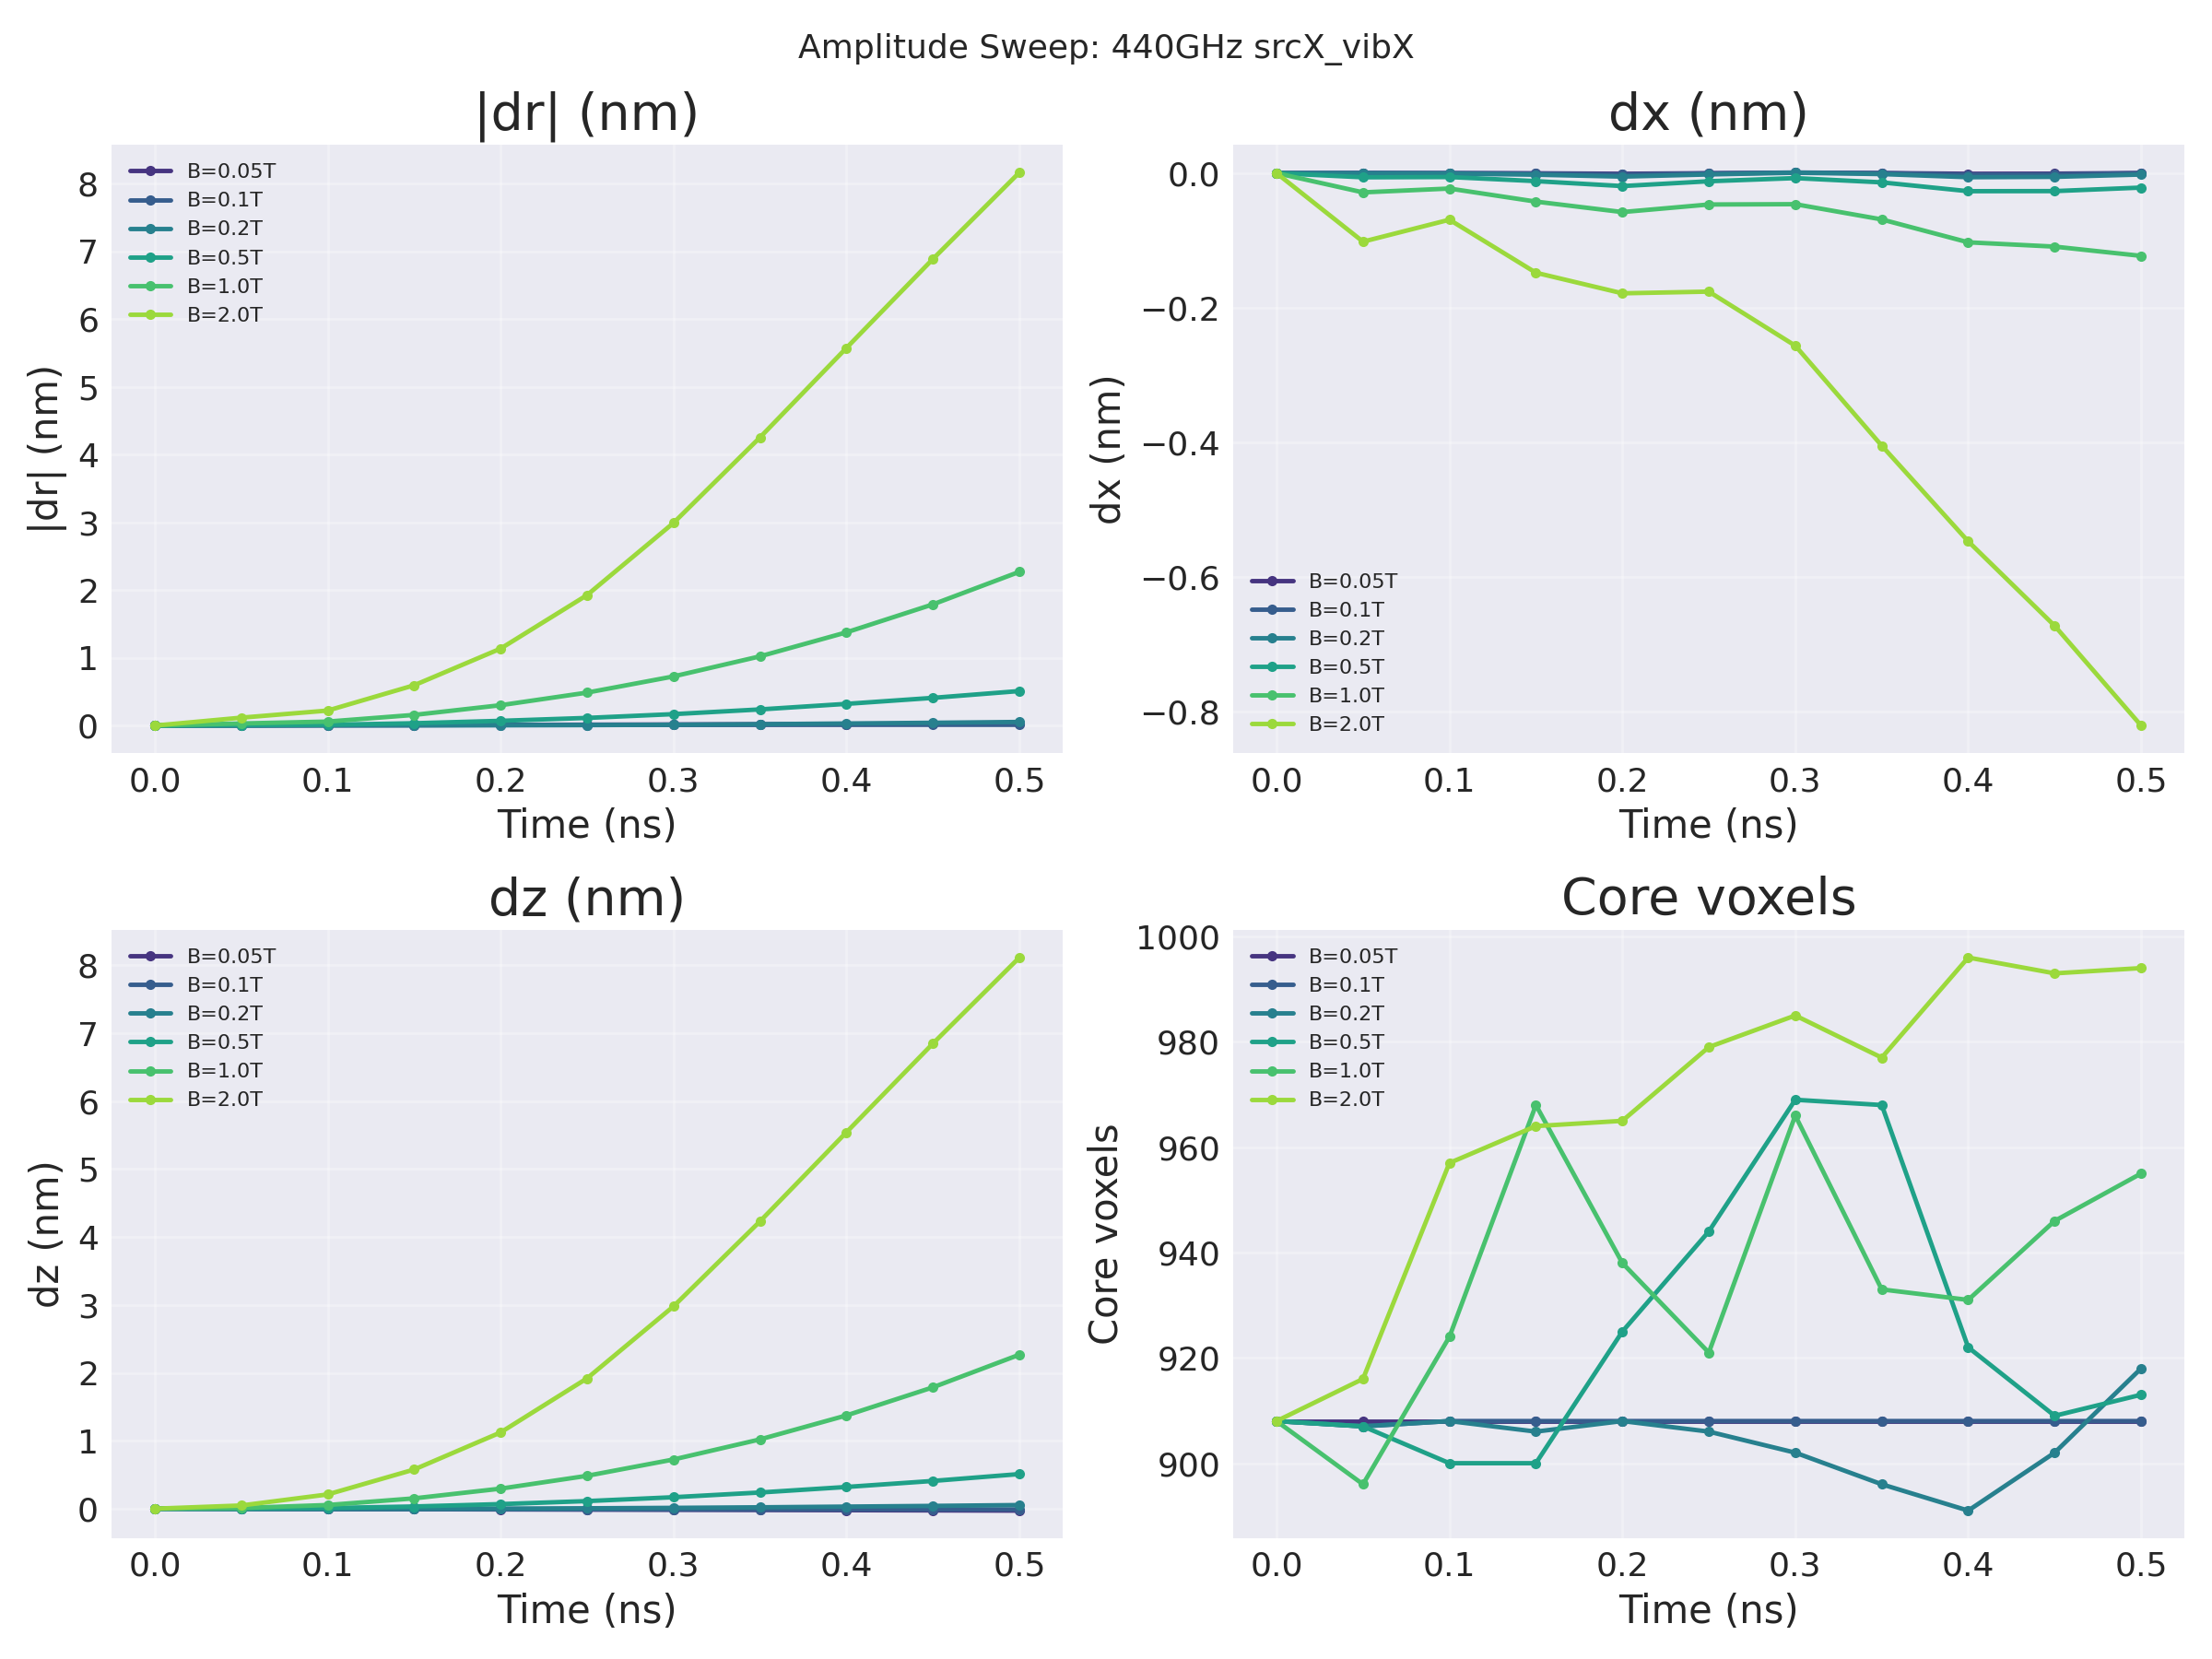
\includegraphics[width=0.95\textwidth]{figures/fig4-8_amplitude_trajectory.png}
  \caption{不同驱动幅度下 Hopfion 质心轨迹对比}
  \label{fig:amplitude-trajectory}
\end{figure}

如\cref{fig:amplitude-scaling}所示，在有效驱动范围内（$B_0 \geq \SI{0.5}{T}$），速度与幅度满足幂律关系：
\begin{equation}
  \bar{v} = A \cdot B_0^n, \quad n = 1.99 \pm 0.01, \quad R^2 = 0.998
  \label{eq:amplitude-scaling}
\end{equation}
指数 $n \approx 2$ 的物理意义是：自旋波携带的线性动量密度正比于能量密度 $\propto B_0^2$，Hopfion 的稳态速度由动量注入率与耗散率的平衡决定，因此 $v \propto B_0^2$。这与 Skyrmion 自旋波驱动中的 $v \propto B_0^2$ 标度律一致\cite{ding2015motion}。

在弱驱动极限（$B_0 \leq \SI{0.1}{T}$），Hopfion 位移降至噪声水平（$|\Delta r| < \SI{0.1}{nm}$），存在阈值效应。$B_0 = \SIrange{0.05}{0.1}{T}$ 时甚至出现反向微弱运动（朝源方向），可能与低幅度下 Hopfion 的弹性反弹效应有关。

\subsection{拓扑 Hall 效应}
\label{subsec:hall-effect}

srcX 驱动下 Hopfion 的运动方向并非沿自旋波传播方向（$+x$），而是几乎垂直于传播方向沿 $+z$ 方向。定义拓扑 Hall 角 $\theta_{\text{H}} = \arctan(v_\perp / v_\parallel)$，其中 $v_\perp$ 为垂直于源平面的速度分量，$v_\parallel$ 为平行于传播方向的分量。

\begin{figure}[htbp]
  \centering
  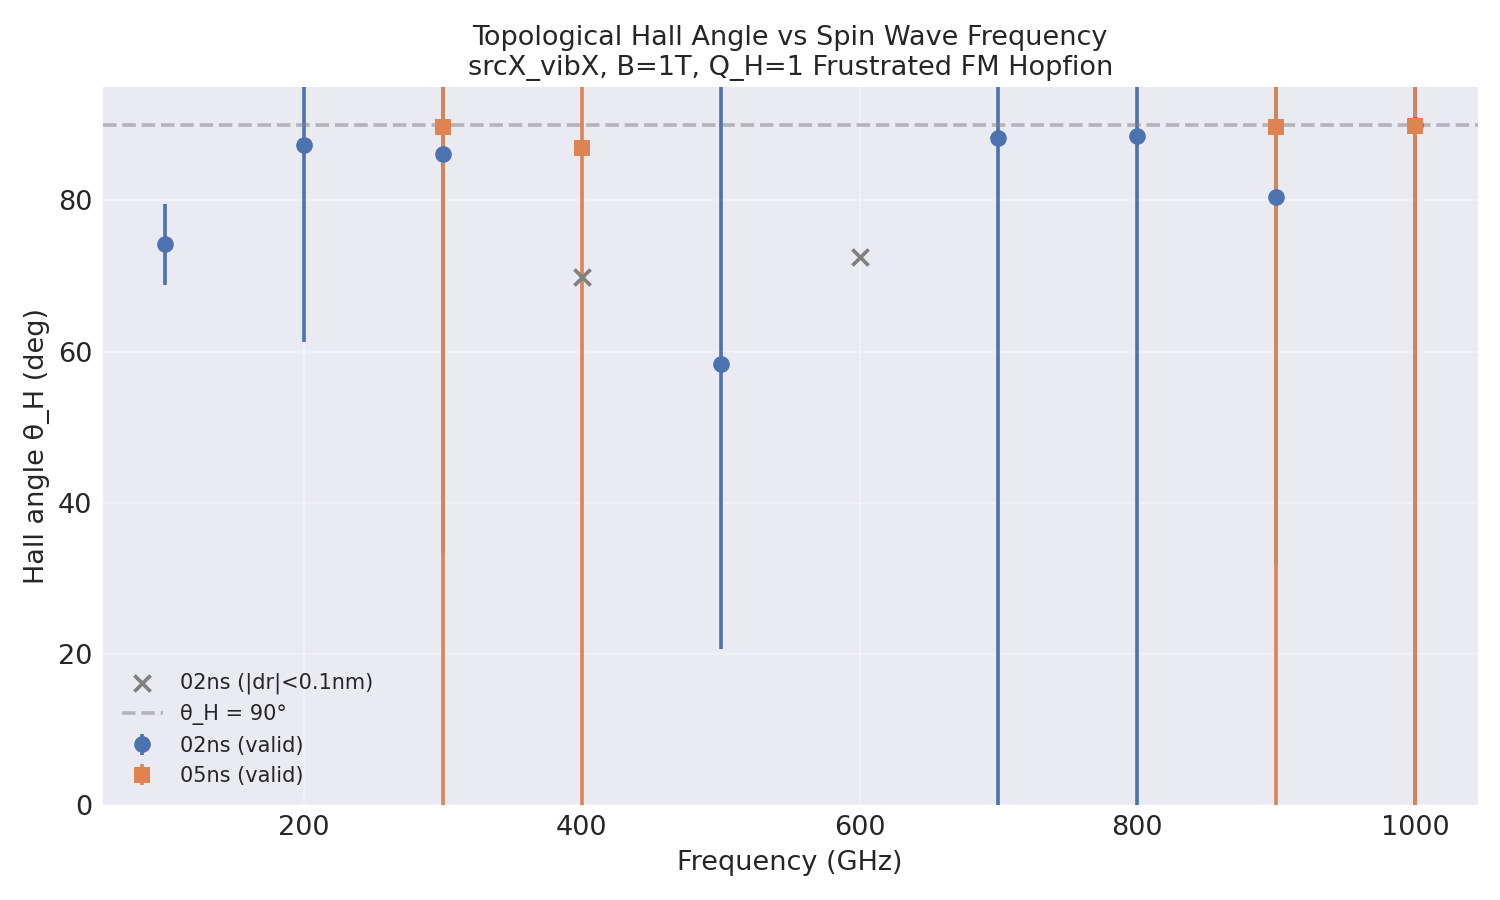
\includegraphics[width=0.95\textwidth]{figures/fig4-9_hall_angle_freq.png}
  \caption{拓扑 Hall 角 $\theta_{\text{H}}$ 随频率的变化。在有效驱动频率下 $\theta_{\text{H}} \approx \ang{87}$--$\ang{90}$，表现出拓扑保护特性}
  \label{fig:hall-angle-freq}
\end{figure}

如\cref{fig:hall-angle-freq}所示，在所有有效驱动频率（$|\Delta r| > \SI{0.3}{nm}$）下，srcX 的 Hall 角均集中在 $\theta_{\text{H}} \approx \ang{87}$--$\ang{90}$，即 Hopfion 几乎完全沿垂直于传播方向运动。

\begin{figure}[htbp]
  \centering
  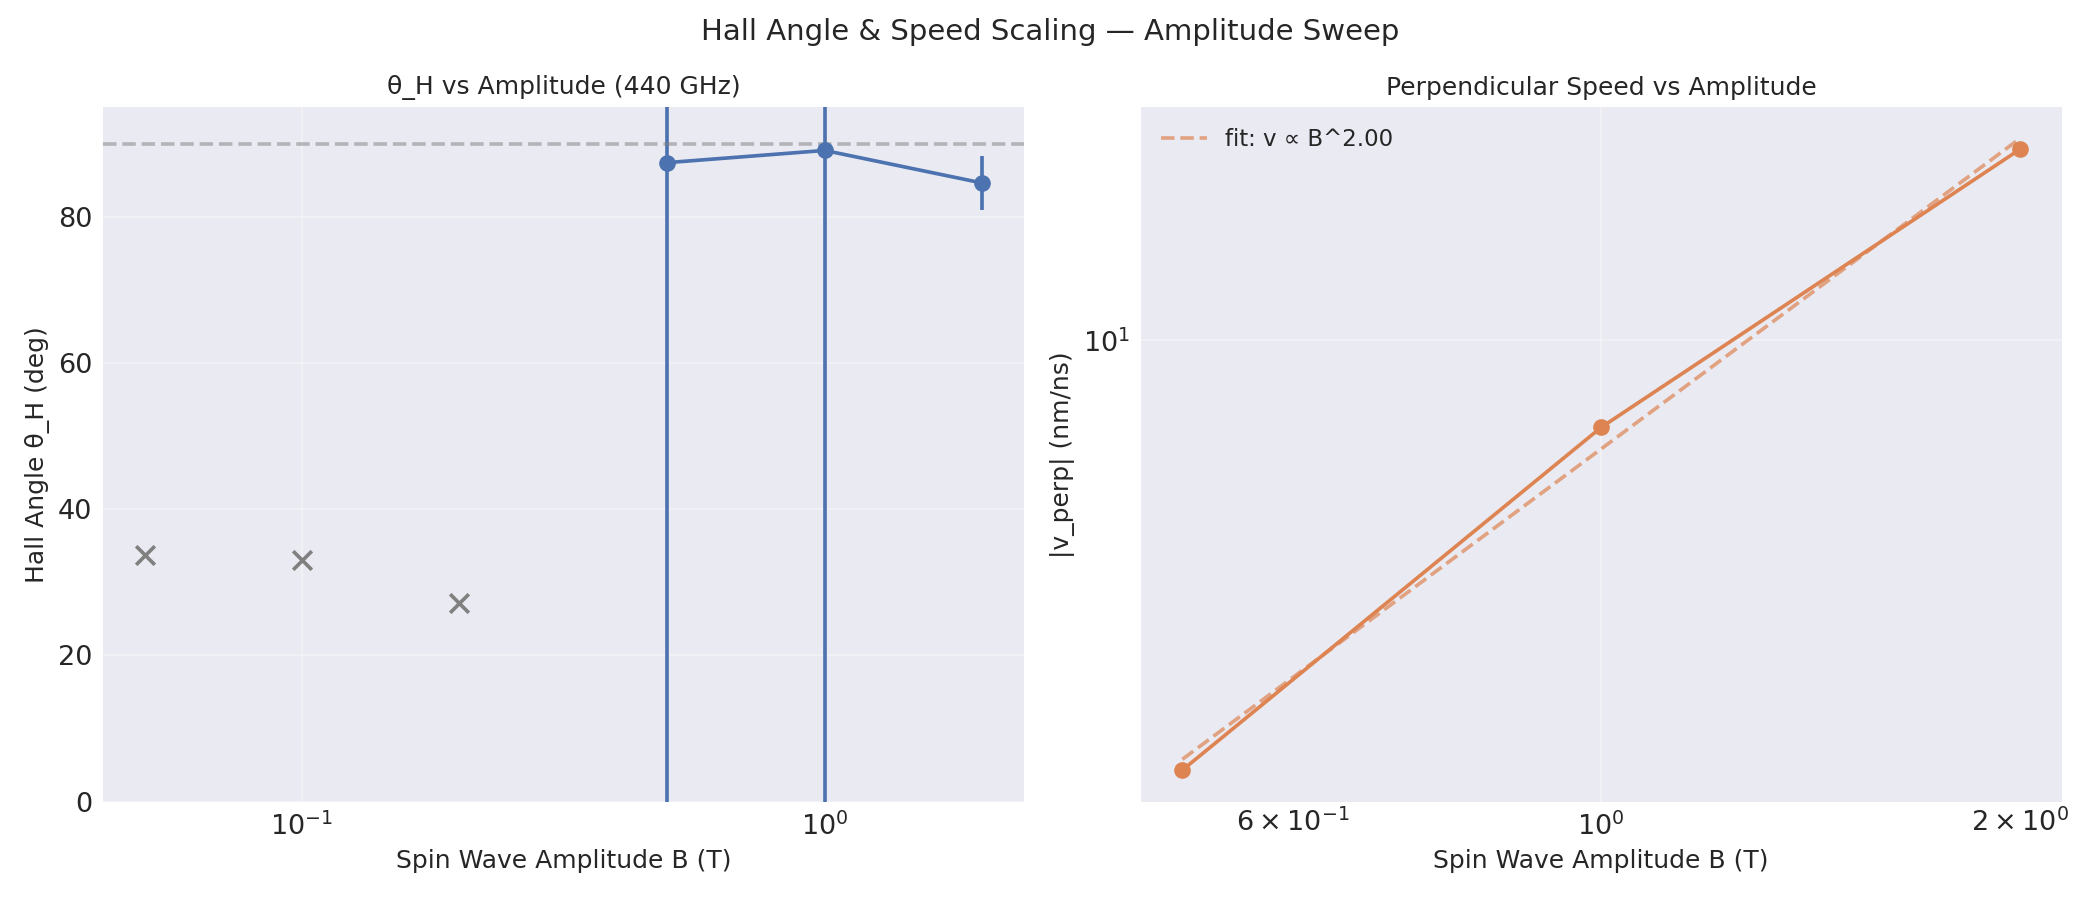
\includegraphics[width=0.95\textwidth]{figures/fig4-9b_hall_angle_amplitude.png}
  \caption{拓扑 Hall 角（左）和垂直速度（右）随自旋波幅度的变化（$f = \SI{440}{GHz}$）。$B_0 \geq \SI{0.5}{T}$ 时 Hall 角锁定在 $\ang{87}$--$\ang{90}$，弱驱动下因位移接近噪声水平而偏离}
  \label{fig:hall-angle-amplitude}
\end{figure}

\cref{fig:hall-angle-amplitude}进一步展示了 Hall 角随驱动幅度的变化。在有效驱动范围（$B_0 \geq \SI{0.5}{T}$）内，Hall 角稳定在 $\ang{87}$--$\ang{90}$，不随幅度变化。这种稳定性同时跨越了频率和幅度两个维度，证实了 Hopfion 磁振子 Hall 效应的拓扑保护特性。也就是说，Hall 角由拓扑结构决定，而不是驱动条件的细节。

相比之下，srcZ 驱动时 Hopfion 沿 $-z$（传播方向）运动，$\theta_{\text{H}} \approx \ang{1}$，Hall 角几乎为零。两种驱动几何下 Hall 角差异很大（srcX 的 $\ang{90}$ vs srcZ 的 $\ang{1}$）。原因是面内自旋波通过动量转移在 Hopfion 位势中产生有效横向力，类似于 Magnus 力在二维 Skyrmion 中的作用\cite{saji2023magnonic}。而轴向自旋波直接沿 Hopfion 对称轴施力，不会激发横向响应。

\subsection{双向轴向控制}
\label{subsec:bidirectional-control}

前述结果表明，srcX 驱动 $+z$ 运动而 srcZ 驱动 $-z$ 运动，且两种驱动的 Hall 角分别为 $\ang{90}$ 和 $\ang{1}$。这意味着通过选择不同的自旋波传播方向，可以实现 Hopfion 沿 $z$ 轴的双向可控运动。更进一步，srcZ 在不同频率下的方向异常（$\SI{100}{GHz}$ 驱动 $+z$ 而 $\SI{1100}{GHz}$ 驱动 $-z$）提供了另一种双向控制策略：单一 srcZ 源通过频率切换即可实现方向反转。

\begin{figure}[htbp]
  \centering
  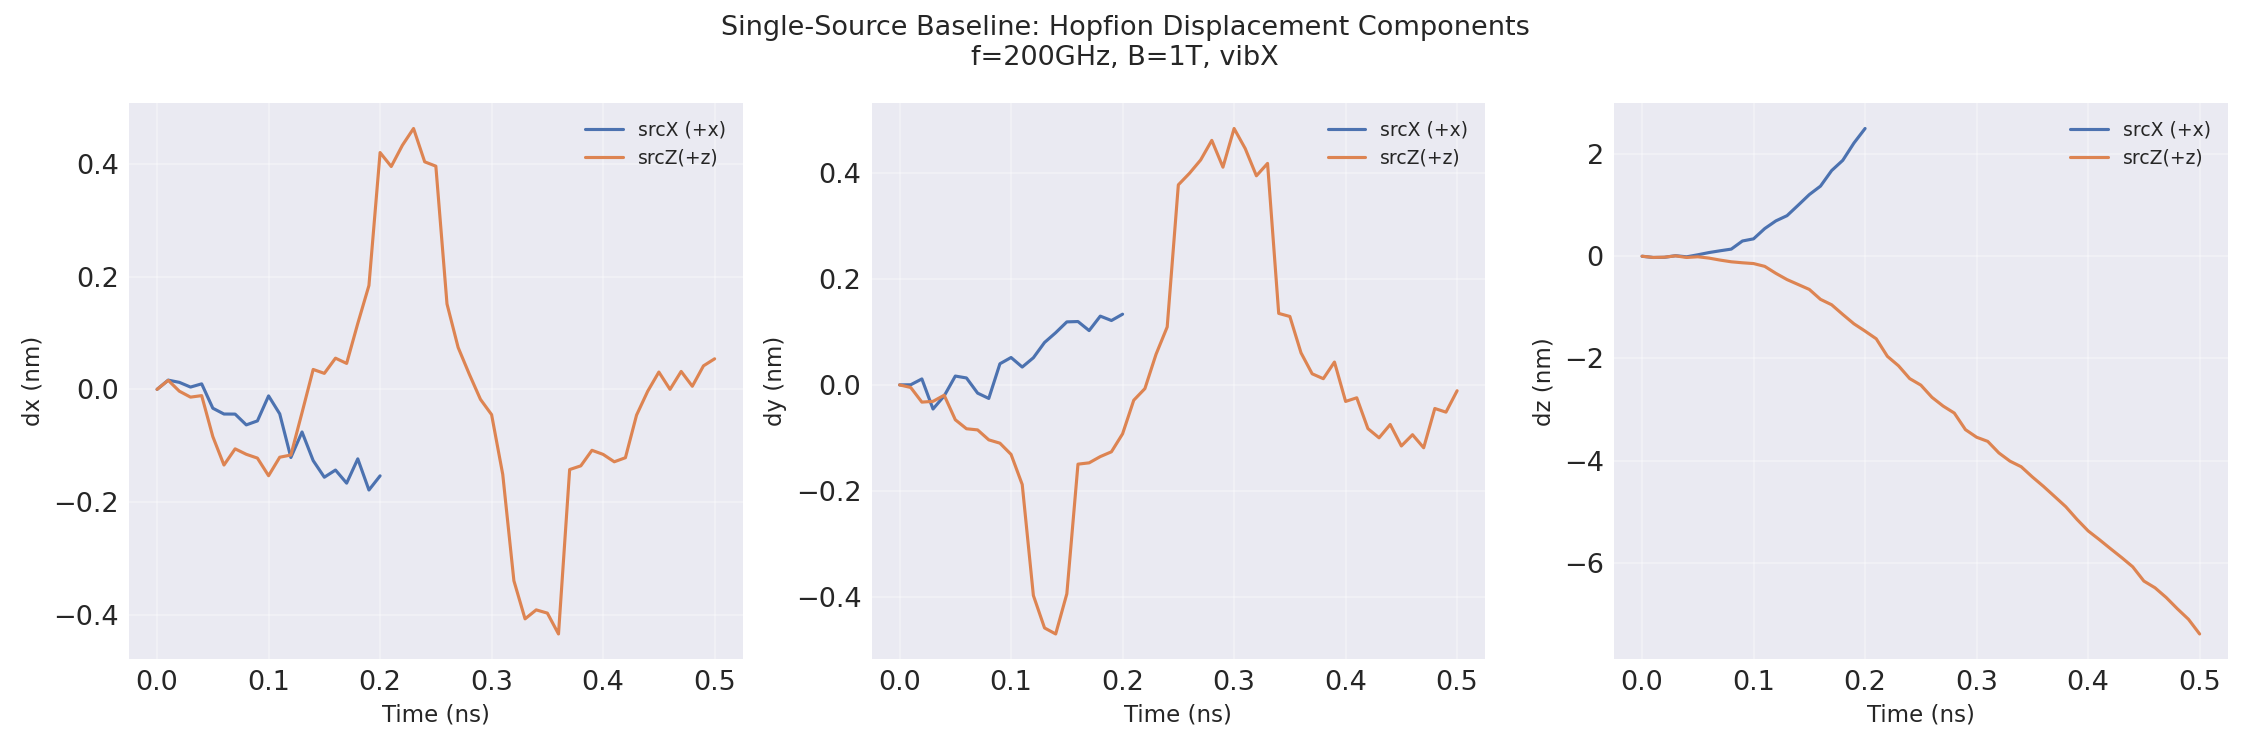
\includegraphics[width=0.95\textwidth]{figures/fig4-10_multisource_baseline.png}
  \caption{三种单源基线的 Hopfion 运动轨迹对比。srcX（$\SI{200}{GHz}$）驱动 $+z$，srcZ（$\SI{200}{GHz}$）驱动 $-z$，Hall 角分别为 $\ang{87}$ 和 $\ang{1}$}
  \label{fig:multisource-baseline}
\end{figure}

\cref{fig:multisource-baseline}展示了 srcX 和 srcZ 单源基线的运动轨迹定量对比，清晰地呈现了两种驱动方向的互补性。

为了验证频率切换方案，本文设计了分时序仿真实验（v3 平衡时序）。Phase~1（$0$--$\SI{0.50}{ns}$）施加 srcZ@$\SI{100}{GHz}$ 驱动 $+z$ 运动，Phase~2（$\SI{0.50}{}$--$\SI{1.00}{ns}$）切换至 srcZ@$\SI{1100}{GHz}$ 驱动 $-z$ 运动。

如\cref{fig:freq-switch-z}所示，Phase~1 中 Hopfion 稳定向 $+z$ 运动，累计位移达 $\SI{+17.6}{nm}$。$\SI{100}{GHz}$ 的 50 个完整周期提供了充足的动量转移。Phase~2 切换至 $\SI{1100}{GHz}$ 后，Hopfion 立即反转为 $-z$ 运动，在约 $\SI{0.41}{ns}$ 内从 $+\SI{17.6}{nm}$ 运动至 $-\SI{12.9}{nm}$（Phase~2 位移 $\SI{-30.5}{nm}$），之后因持续强驱动导致 Hopfion 结构失稳而坍塌。

这一实验证实了单一 srcZ 源通过频率切换可以实现 Hopfion 运动方向的完全反转。$-z$ 方向的速度（$\sim\SI{74}{nm/ns}$）远高于 $+z$（$\sim\SI{35}{nm/ns}$），说明两种频率的耦合强度不同。Hopfion 在 Phase~2 后期的坍塌表明，强自旋波驱动下拓扑结构的寿命是有限的。实际应用中需要优化驱动幅度或引入脉冲调制，以兼顾速度和寿命。

\begin{figure}[htbp]
  \centering
  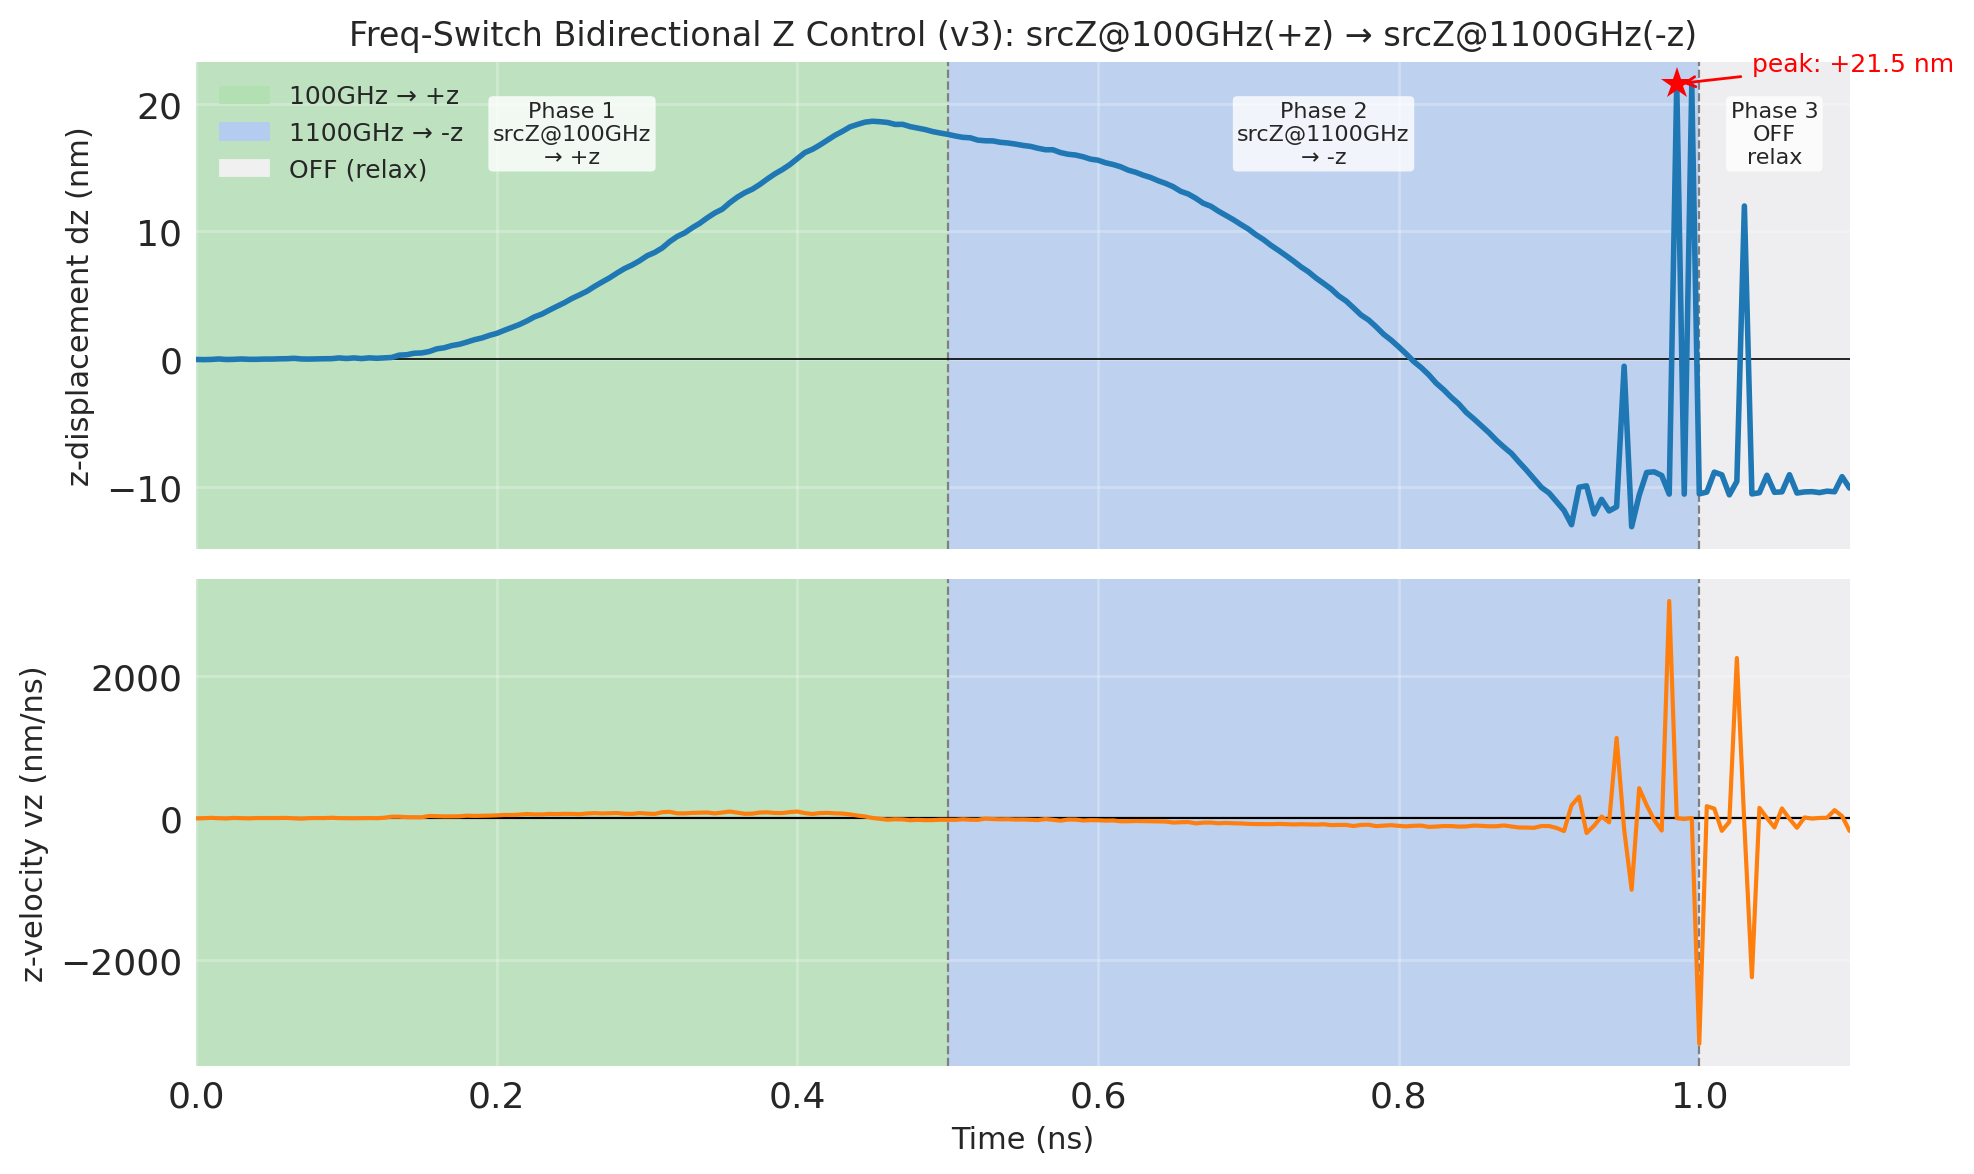
\includegraphics[width=0.95\textwidth]{figures/fig4-11_freq_switch_z_control.png}
  \caption{频率切换双向 $z$ 轴控制验证（v3 平衡时序）。上：$z$ 方向位移随时间变化；下：$z$ 方向速度。绿色区域为 srcZ@$\SI{100}{GHz}$（$0$--$\SI{0.50}{ns}$，$+z$），蓝色区域为 srcZ@$\SI{1100}{GHz}$（$\SI{0.50}{}$--$\SI{1.00}{ns}$，$-z$）。Hopfion 在 $t \approx \SI{0.91}{ns}$ 因强驱动而坍塌}
  \label{fig:freq-switch-z}
\end{figure}

\subsection{与二维 Skyrmion 自旋波驱动的对比}

Hopfion 的自旋波驱动机制可与二维 Skyrmion 的情况进行类比。Ding 等人\cite{ding2015motion}和 Huang 等人\cite{huang2023transient}发现，自旋波通过线性动量转移驱动 Skyrmion 沿传播方向运动，且运动速度与自旋波频率和振幅相关。Shen 等人\cite{shen2018skyrmionium}研究了回旋矢量为零的 Skyrmionium 在自旋波驱动下的运动，发现其沿自旋波传播方向直线运动而无霍尔偏转——这与 Hopfion 的 $\mathbf{G} = 0$ 特性形成直接类比。

本章仿真结果与上述二维体系的主要异同总结如下：

\begin{enumerate}
  \item \textbf{幅度标度律一致}：Hopfion 的 $v \propto B_0^{1.99}$ 与 Skyrmion/Skyrmionium 的 $v \propto B_0^2$ 一致，确认三维拓扑结构中动量转移的基本机制不变。
  \item \textbf{Hall 角差异}：二维 Skyrmion 的 Hall 角取决于拓扑荷 $Q$ 和耗散张量，通常为 $\ang{0}$--$\ang{60}$。而 Hopfion 的 srcX 驱动产生 $\theta_{\text{H}} \approx \ang{90}$，这一极端 Hall 角在二维体系中罕见，反映了三维拓扑结构的特殊耦合机制。Saji 等人\cite{saji2023magnonic}从解析角度预测了类似的磁振子 Hall 效应，本章仿真首次在微磁学层面给出定量验证。
  \item \textbf{三维新自由度}：二维 Skyrmion 仅有面内运动，而 Hopfion 的三维结构提供了额外的轴向自由度。srcX 和 srcZ 分别激发面内-轴向耦合和直接轴向运动，使得单一体系中可实现双向控制——这是二维拓扑结构无法实现的功能。
  \item \textbf{振荡方向选择性}：二维体系中自旋波的面内/面外振荡均可驱动 Skyrmion\cite{ding2015motion}，而 Hopfion 仅响应面内振荡，面外振荡完全无效。这一选择性源于 Hopfion 的轴对称拓扑结构。
\end{enumerate}

\subsection{点源与平面源的对比}
\label{subsec:point-vs-plane}

前述实验均采用平面波激励（$\SI{0.5}{nm}$ 厚薄片层，$B_0 = \SI{1}{T}$）。为了考察激励几何对驱动行为的影响，本文设计了点源对照实验。激励区域缩小为单个网格单元（$\SI{0.5}{nm}^3$，位于同一坐标），幅度提高至 $B_0 = \SI{500}{T}$ 以补偿体积差异，其余参数不变。本文对 srcX 和 srcZ 两种传播方向分别进行了 $\SIrange{100}{1000}{GHz}$ 的 10 点频率扫描。

\begin{figure}[htbp]
  \centering
  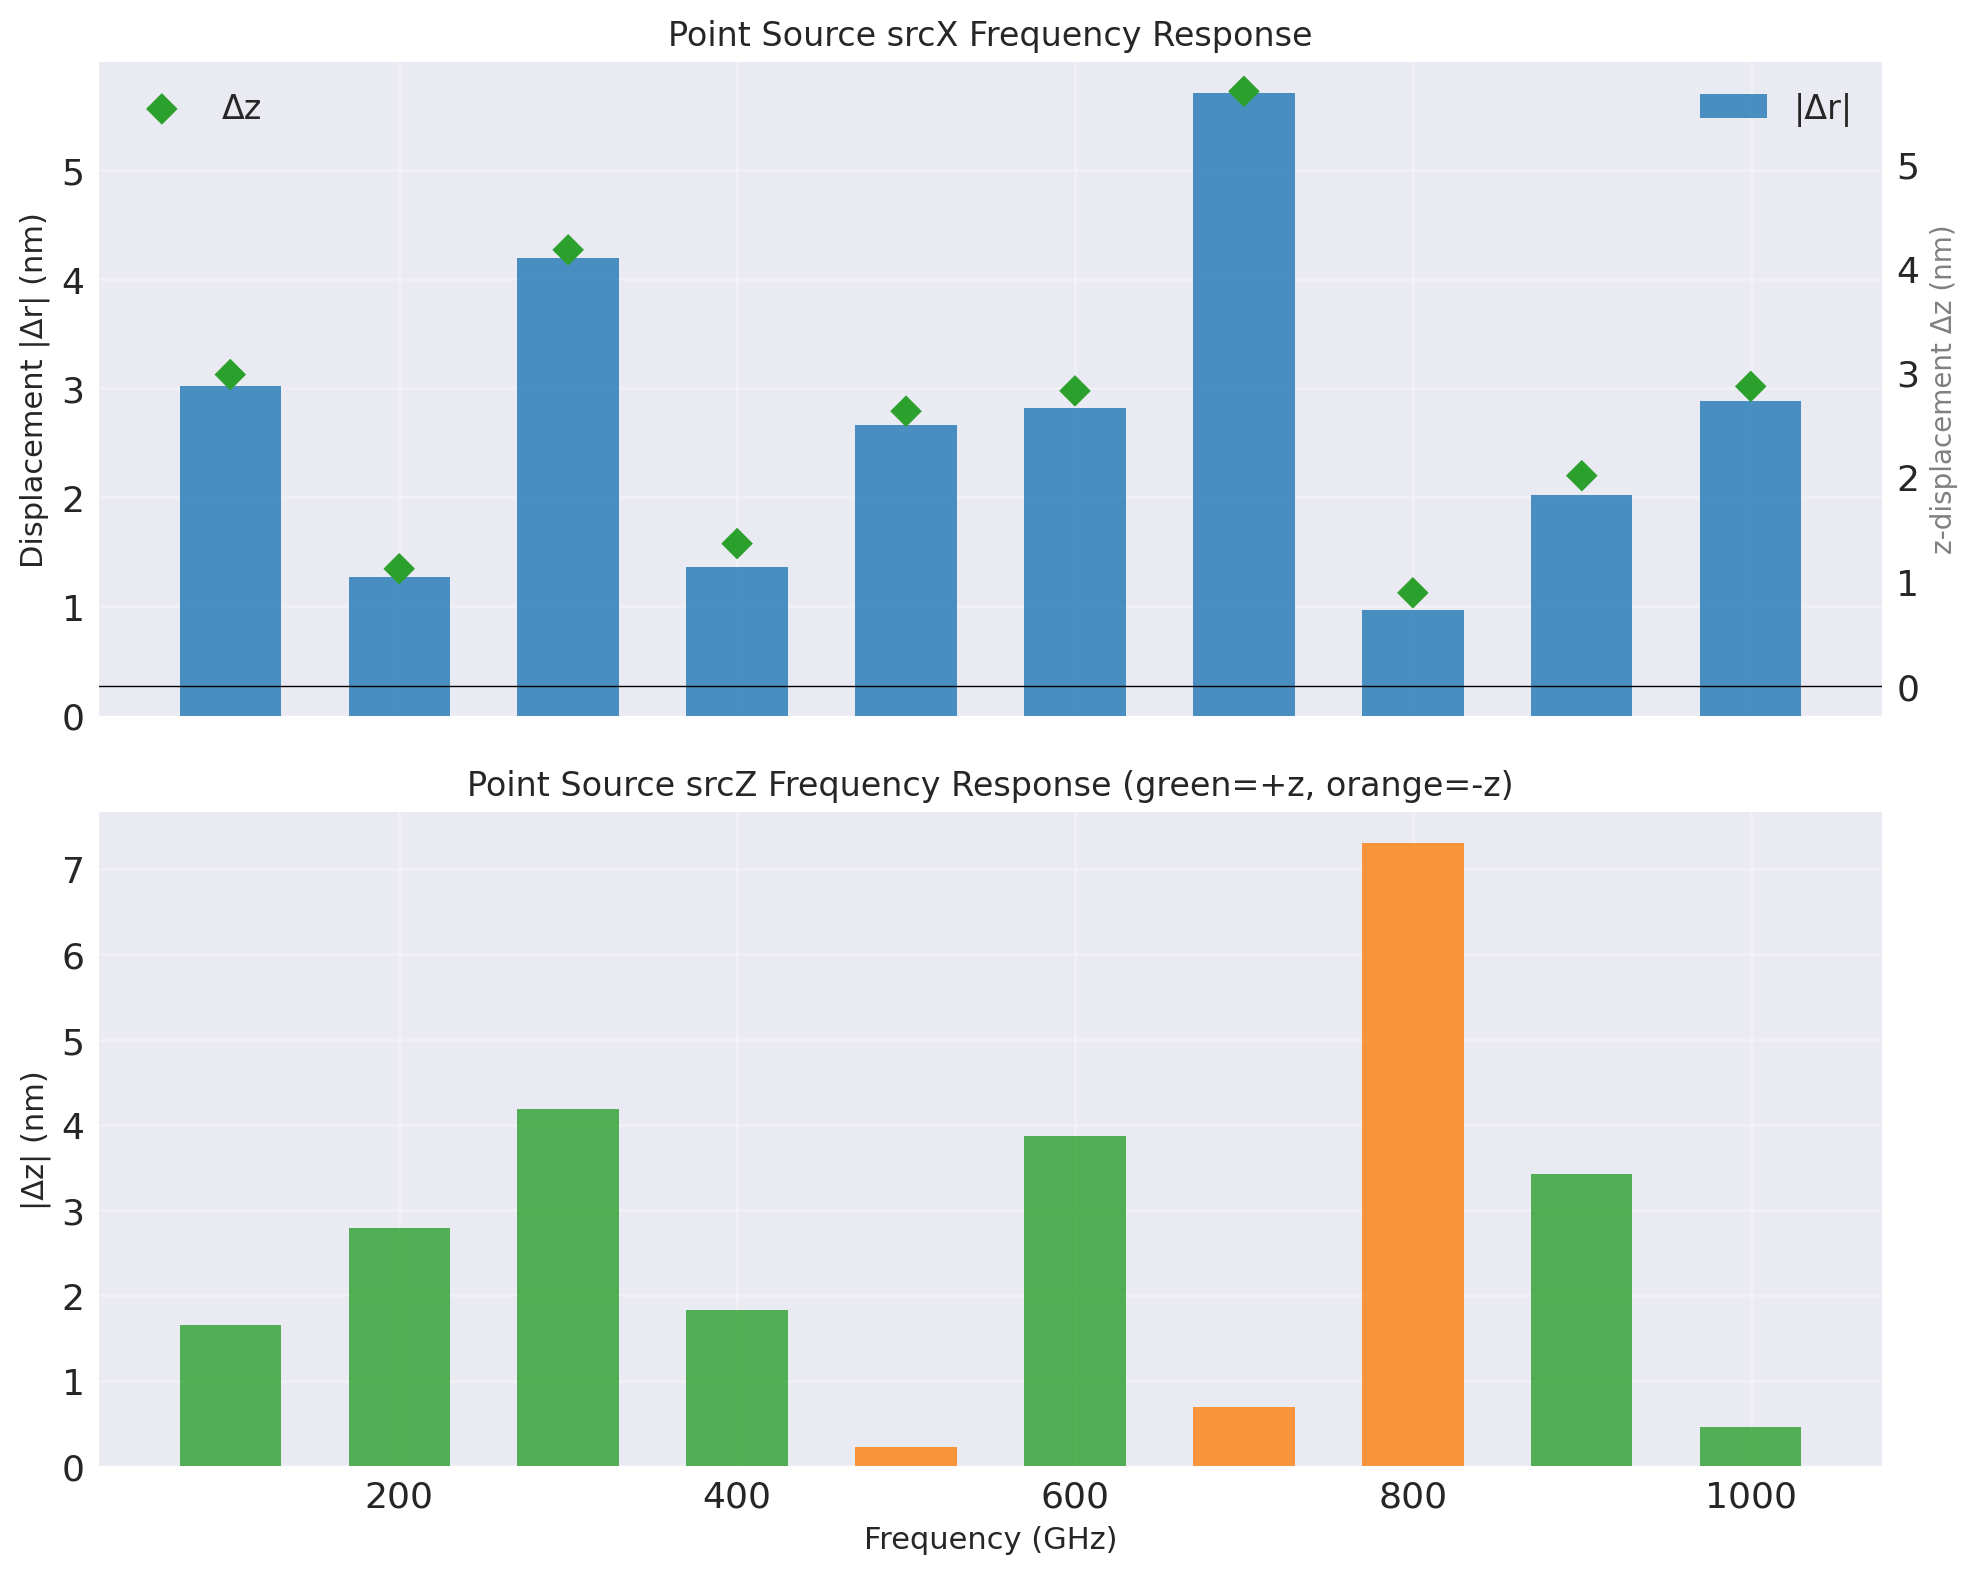
\includegraphics[width=0.95\textwidth]{figures/fig4-12_point_source_freq_response.png}
  \caption{点源驱动的频率响应谱。上：srcX，$\SI{700}{GHz}$ 最强（$|\Delta r| = \SI{5.7}{nm}$）；下：srcZ，$\SI{800}{GHz}$ 最强（$|\Delta r| = \SI{7.3}{nm}$，$-z$），绿色/橙色分别对应 $+z$/$-z$ 运动方向}
  \label{fig:point-source-freq}
\end{figure}

如\cref{fig:point-source-freq}所示，点源驱动与平面源呈现显著差异：

\begin{enumerate}
  \item \textbf{共振频率偏移}：srcX 的最强响应从平面源的 $\SI{1000}{GHz}$ 偏移至 $\SI{700}{GHz}$（$|\Delta r| = \SI{5.7}{nm}$），死区消失；srcZ 的最强响应从 $\SI{1100}{GHz}$ 偏移至 $\SI{800}{GHz}$（$|\Delta r| = \SI{7.3}{nm}$）。这一偏移可归因于点源激发的自旋波包含更宽的波矢分布，与 Hopfion 内部模式的耦合条件发生变化。
  \item \textbf{方向特征保持}：srcX 点源在所有 10 个频率下均驱动 $+z$ 运动，与平面源一致。srcZ 的方向分布更为复杂——100--$\SI{400}{GHz}$、$\SI{600}{GHz}$ 和 $\SI{900}{GHz}$ 为 $+z$，$\SI{500}{GHz}$、$\SI{700}{GHz}$ 和 $\SI{800}{GHz}$ 为 $-z$——相比平面源仅 $\SI{100}{GHz}$ 异常，点源中多个频率出现方向反转。
  \item \textbf{Hall 角鲁棒性}：如\cref{fig:point-source-hall}所示，srcX 点源的 Hall 角仍集中在 $\ang{69}$--$\ang{89}$，保持了高 Hall 角的拓扑特征。srcZ 的 Hall 角从平面源的 $\approx\ang{1}$ 增大至 $\ang{9}$--$\ang{40}$，说明点源的非对称激励部分打破了轴向对称性，引入了微弱的横向耦合。
\end{enumerate}

\begin{figure}[htbp]
  \centering
  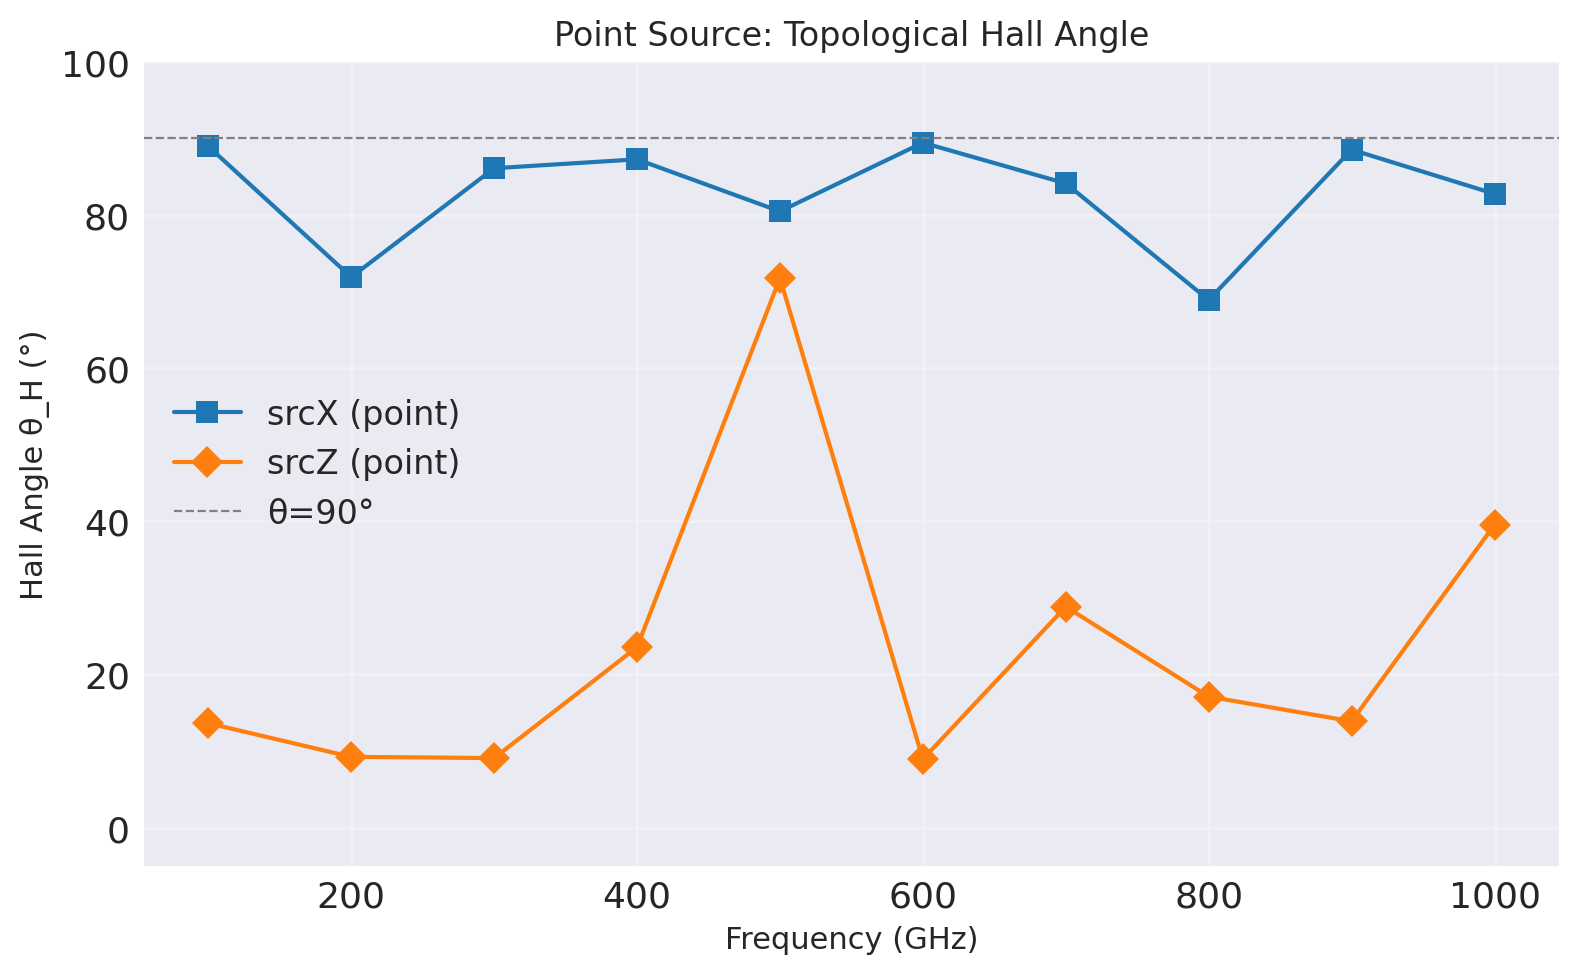
\includegraphics[width=0.85\textwidth]{figures/fig4-13_point_source_hall_angle.png}
  \caption{点源与平面源的 Hall 角对比。srcX 的高 Hall 角（$\ang{69}$--$\ang{89}$）保持不变，srcZ 从 $\approx\ang{1}$ 增至 $\ang{9}$--$\ang{40}$}
  \label{fig:point-source-hall}
\end{figure}

上述对比表明，Hopfion 对自旋波的响应特征——振荡方向选择性、运动方向、高 Hall 角——本质上由 Hopfion 的拓扑结构决定，和激励几何的细节无关。点源虽然改变了共振频率分布和方向分布的细节，但没有改变基本的物理图像。


\section{本章小结}

本章系统研究了自旋波驱动 Hopfion 运动的物理机制，主要结论如下：

\begin{enumerate}
  \item \textbf{方向选择性}：只有面内振荡（vibX）的自旋波才能有效驱动 Hopfion 运动，面外振荡（vibZ）无效。面内传播（srcX/srcY）具有各向同性，验证了 Hopfion 的轴对称性。
  \item \textbf{频率响应}：srcX 在 $\SI{1000}{GHz}$ 有最强响应（$|\Delta r| = \SI{5.5}{nm}$），死区为 $\SIrange{400}{600}{GHz}$。srcZ 在 $\SI{1100}{GHz}$ 响应最强（$|\Delta r| = \SI{18.1}{nm}$），并呈现多峰共振谱。srcZ 在 $\SI{100}{GHz}$ 出现方向异常（$+z$），其余频率均为 $-z$。
  \item \textbf{幅度标度律}：Hopfion 运动速度与自旋波幅度满足 $v \propto B_0^{1.99}$（$R^2 = 0.998$），符合动量转移理论预期。
  \item \textbf{拓扑 Hall 效应}：srcX 驱动产生 $\theta_{\text{H}} \approx \ang{87}$--$\ang{90}$ 的 Hall 角，在不同频率和幅度下高度稳定，体现拓扑保护特性。srcZ 的 Hall 角 $\approx \ang{1}$，几乎沿传播方向运动。
  \item \textbf{双向控制}：srcX（$+z$）和 srcZ（$-z$）的方向互补性，以及 srcZ 的频率依赖方向异常，为实现 Hopfion 的 $z$ 轴双向可控运动提供了两种可行方案。
  \item \textbf{激励几何鲁棒性}：点源与平面源对比表明，Hopfion 的振荡方向选择性和高 Hall 角等核心特征由拓扑结构决定，不依赖于激励几何细节。
\end{enumerate}
